% body
\section{Results\label{sec:results}}
We now demonstrate the accuracy and performance of \qbkix to evaluate singular/near-singular layer potentials on various complex geometries to solve the integral equation in \cref{eq:int-eq} and evaluate the solution as defined in \cref{eq:double_layer}.

\subsection{Classical convergence with patch refinement}
We will first demonstrate the numerical convergence behavior of \qbkix.
As discussed in \cite[Section 3.1]{KBGN}, approximation-based schemes such as \qbkix do not converge classically but do so up to a controlled precision if $r$ and $R$ scale with proportional to the patch size. 
In order to observe classical convergence as we refine $\Pcoarse$, we must allow $R$ and $r$ to decrease slower than $O(L)$, such as with rate $O(\sqrt{L})$.
In this section, we choose the \qbkix parameters $a$ and $b$ proportional to $1/\sqrt{L}$ to achieve this and demonstrate numerical convergence with refinement of $L$.

In our examples, we use analytic solutions to \cref{eq:pde} obtained as sums of point charge functions of the form 
\begin{equation}
  u_c(\vx) = \sum_{i=1}^m G(\vx,\vy_i)\psi_i
  \label{eq:point-charge-solution}
\end{equation}
%are solutions to \cref{eq:pde} by construction, 
where the charge locations $\vy_i$ with strengths $\psi_i$ are outside of $\Omega$.
To construct specific solutions, we sample a sphere of radius one with point charges, as shown in \Cref{fig:greens-id-test-cases,fig:solver-conv-test-cases}.
We choose charge strengths $\psi_i$ randomly from $[0,1]^d$, where $d=1$ for Laplace problems and $d=3$ for Stokes and elasticity problems. 

We use the multipole order  $m=20$ with $5000$ points per leaf box for the  kernel-independent \fmm. 
This ensures that the \fmm error does not dominate;  sufficiently large number of points per leaf box is needed to minimize the additional error due to tree depth.
We choose a high quadrature order $q=20$, or 400 quadrature points per patch in $\Pcoarse$, relative to overall convergence order to satisfy the assumption in \cref{sec:adaptive_upsampling}.
We also use two levels of uniform upsampling to demonstrate convergence.


\subsubsection{Green's Identity}
\begin{figure}[!htb]
  \centering
  \begin{minipage}{.5\textwidth}
      \centering
    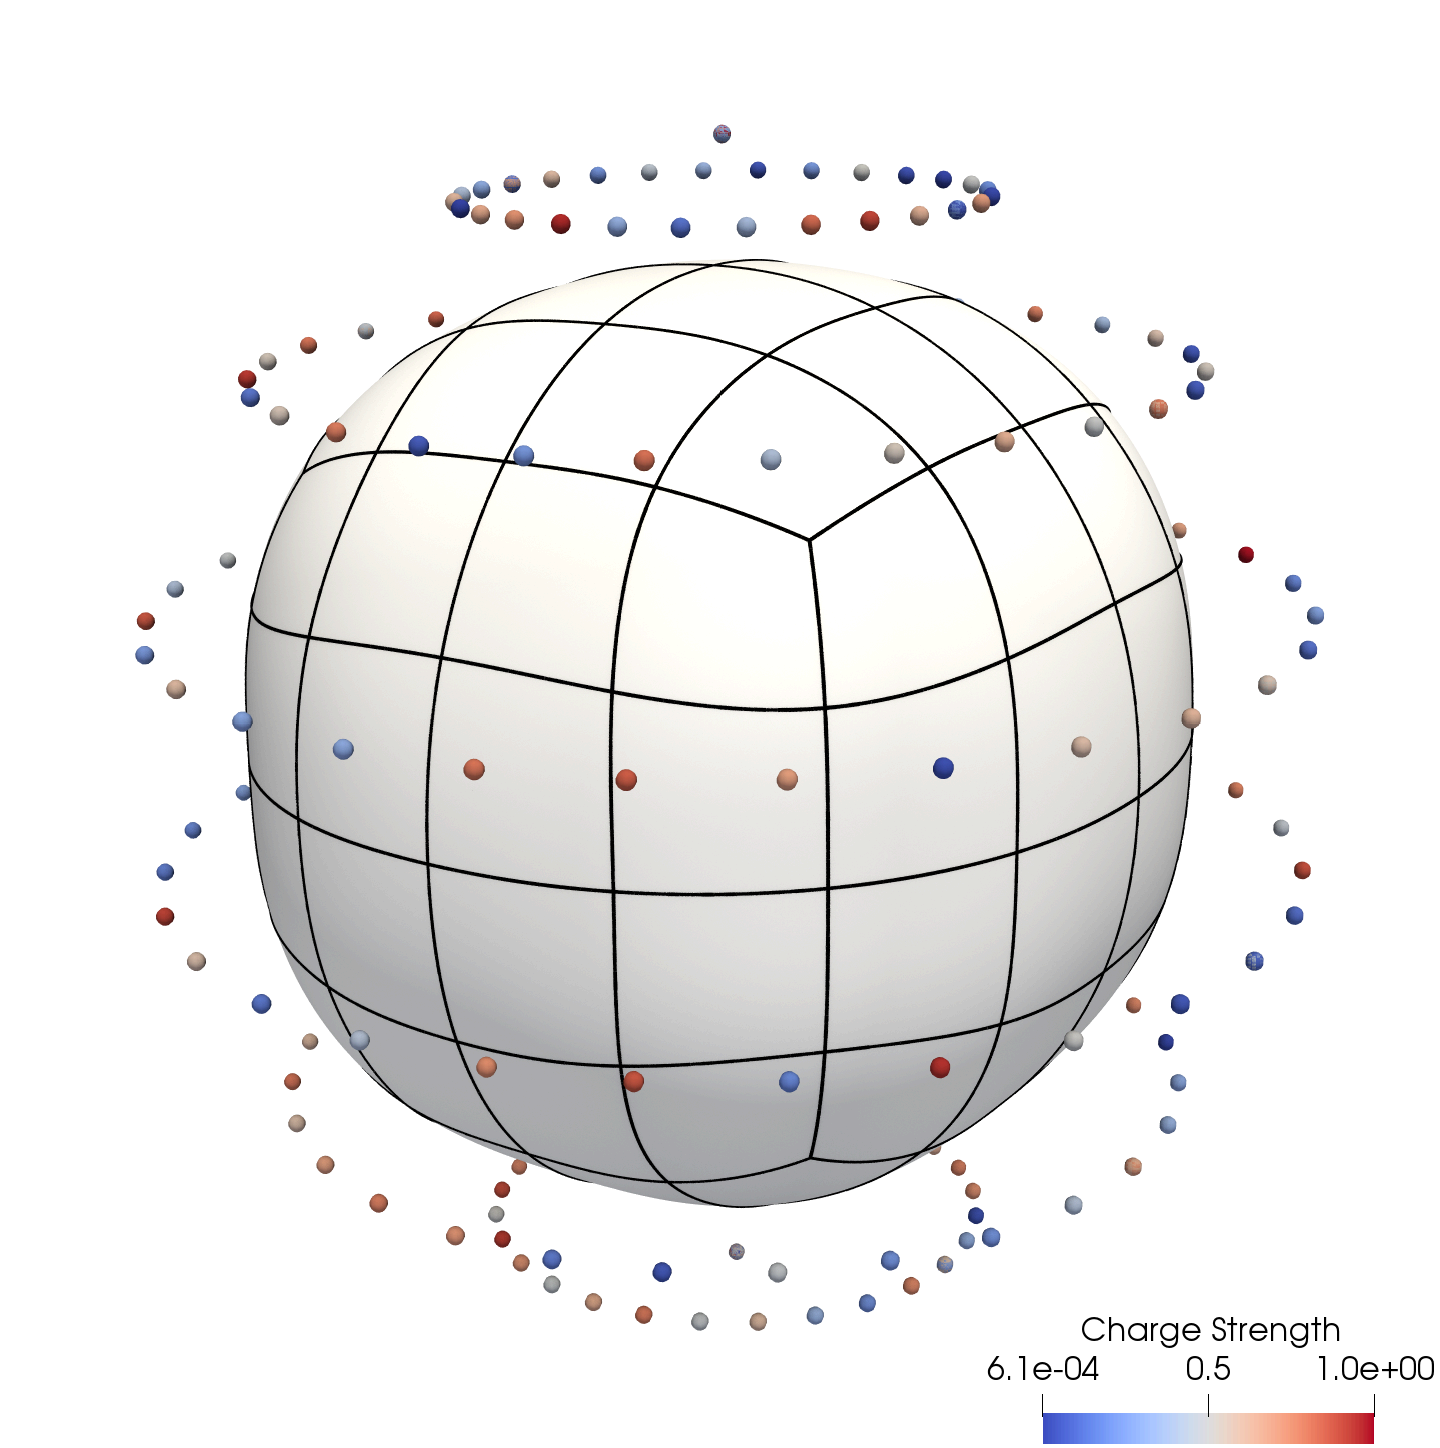
\includegraphics[width=.75\linewidth]{figs/cube_convergence_setup}
  \end{minipage}\hfill
  \begin{minipage}{.5\textwidth}
      \centering
    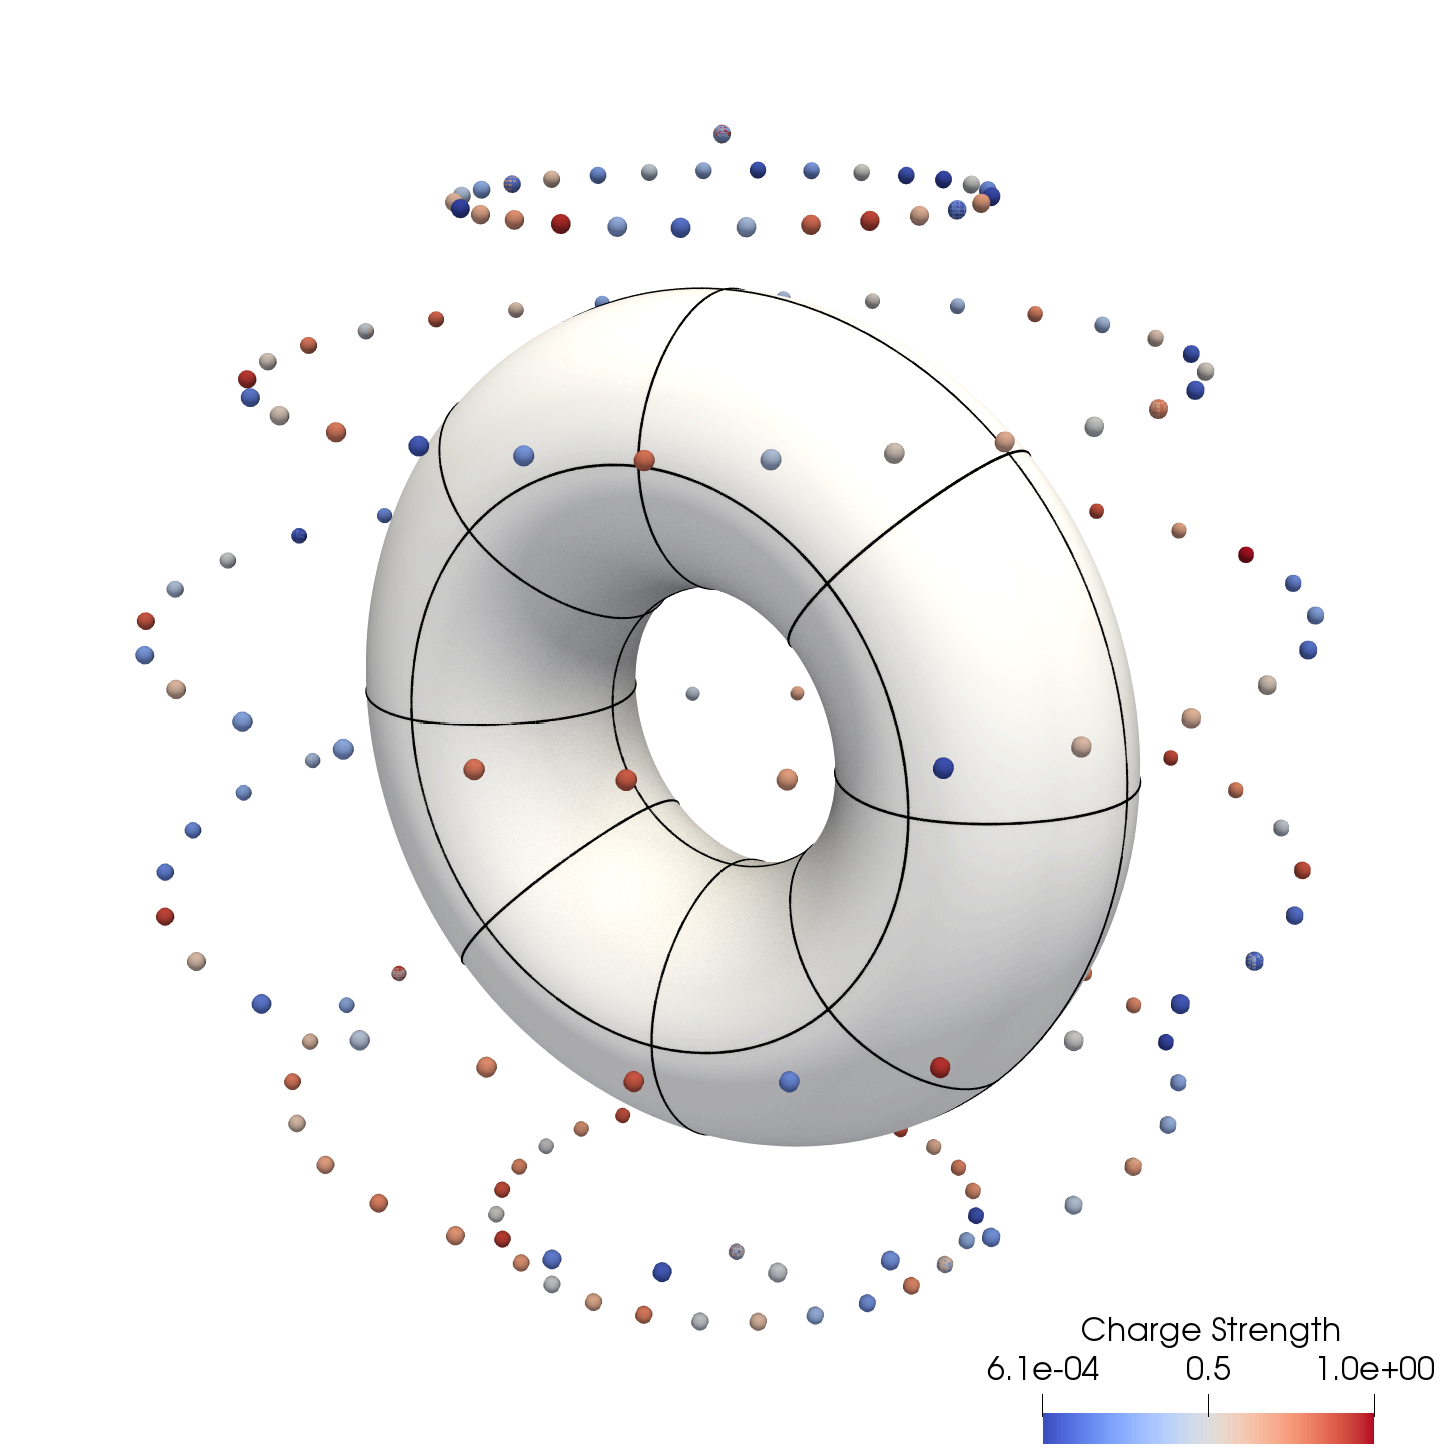
\includegraphics[width=.75\linewidth]{figs/newtorus_convergence_setup}
  \end{minipage}\hfill
  \mcaption{fig:greens-id-test-cases}{}{Geometry and singularities used for Green's Identity convergence tests. 
  Shown are polynomial patches defining boundary geometry (black lines) and point singularities
  placed on the surface on a sphere of radius one.
  Singularity strengths are randomly selected values in $[0,1]$; shown is the strength intensity for Laplace problems, which varies from blue to red.
  We use 96 20th-order polynomial patches for the spheroid (left) and 32 cubic patches for the torus (right).
}
\end{figure}

\begin{table}[!htb]
\centering
\small
\setlength\tabcolsep{4pt}
\begin{tabular}{lllllll}
\toprule
{}Geometry & \pde &\multicolumn{4}{c}{Relative $\ell^\infty$ error (Number of patches)} & EOC\\
\midrule
Spheroid                                    & Laplace         &  $1.06\times 10^{-4}$ (96) &  $4.78\times 10^{-6}$ (384) &  $9.14\times 10^{-8}$ (1536) &  $4.35\times 10^{-9}$ (6144) & 4.77\\
(\cref{fig:greens-id-test-cases}-left)  & Elasticity      &  $1.68\times 10^{-3}$ (96) &  $6.94\times 10^{-5}$ (384) &  $1.53\times 10^{-6}$ (1536) &  $1.33\times 10^{-8}$ (6144) & 5.74\\
                                        & Stokes          &  $1.92\times 10^{-3}$ (96) &  $7.95\times 10^{-5}$ (384) &  $1.74\times 10^{-6}$ (1536) &  $1.53\times 10^{-8}$ (6144) & 5.72 \\
 \midrule
Torus                                         & Laplace         &  $2.05\times 10^{-3}$ (32) &  $7.52\times 10^{-5}$ (128) &   $3.79\times 10^{-6}$ (512) &  $8.48\times 10^{-8}$ (2048) & 5.45\\
 (\cref{fig:greens-id-test-cases}-right)      & Elasticity      &  $4.38\times 10^{-2}$ (32) &  $1.17\times 10^{-3}$ (128) &   $5.08\times 10^{-5}$ (512) &  $1.42\times 10^{-6}$ (2048) & 5.09\\
                                              & Stokes          &  $5.03\times 10^{-2}$ (32) &  $1.33\times 10^{-3}$ (128) &   $5.81\times 10^{-5}$ (512) &  $1.65\times 10^{-6}$ (2048) & 5.09\\
\bottomrule
\end{tabular}
\mcaption{table:greens-id-data}{$\ell^\infty$ Relative error in Green's Identity versus number of patches}{
  The solution to \cref{eq:pde} due to a known function $u_c$, shown in \cref{fig:greens-id-test-cases} is computed via Green's Identity.
  We evaluate the single- and double-layer potentials with \qbkix due to the Dirichlet and Neumann boundary data and compare against the known value of $u_c$ on the boundary.
  Each column is the result of an additional level of uniform quadrisection of the patches in $\Pcoarse$. 
  The final column (EOC) is the estimated convergence order, computed via least-squares log-log fit of the error as a function of max patch size.
}
\end{table}

We report the accuracy of the \qbkix evaluation scheme in \cref{table:greens-id-data}, where we verify Green's Identity for a random known function $u_c$ in \cref{eq:point-charge-solution}.
We evaluate the Dirichlet and Neumann boundary data due to $u_c$ at the discretization points of $\Gammah$ and use one-sided \qbkix to evaluate the corresponding single- and double-layer potentials at the same discretization points.
With each column of \cref{table:greens-id-data}, we subdivide $\Pcoarse$ to more accurately resolve the boundary condition.
The error shown in \cref{table:greens-id-data} is the $\ell^\infty$-relative error in the solution value
\begin{equation}
  \frac{\left\|\hat{S}\left[\frac{\partial u_c}{\partial \vn}\right](\vx) - \hat{D} \left[ u_c \right](\vx) - u_c(\vx)\right\|_\infty}{\|u_c\|_\infty},
\end{equation}
where $\hat{S}$ and $\hat{D}$ are the single- and double-layer singular integral operators discretized and evaluated with \qbkix.
In these tests, we choose $p=6$, $r=.004\sqrt{L}$ ($a=.004/\sqrt{L}$) and $R=.03\sqrt{L}$ ($b=.03/\sqrt{L}$).
We observe roughly $5$th order convergence on both the spheroid and torus test geometries in \cref{fig:greens-id-test-cases} for each of the tested \pde's.
In \cref{table:greens-id-perf-data}, we present the number of target points evaluated per second per core with one-sided \qbkix. 
We see that performance is best for Laplace and worst for elasticity problems, as expected. 
\begin{table}[!htb]
\centering
\small
\setlength\tabcolsep{8pt}
\begin{tabular}{llllll}
\toprule
{}Geometry & \pde &\multicolumn{4}{c}{Target points/second/core}\\
\midrule
Spheroid                                    & Laplace         &  $3684$ &  $5438$ &  $5077$ &  $5629$ \\
(\cref{fig:greens-id-test-cases}-left)  & Elasticity      &  $1325$ &  $1731$ &  $1687$ &  $1790$ \\
                                        & Stokes          &  $1635$ &  $2075$ &  $2016$ &  $2120$ \\
 \midrule
Torus                                         & Laplace         &  $2729$  &  $3373$ &   $4564$  &  $5477$ \\
 (\cref{fig:greens-id-test-cases}-right)      & Elasticity      &  $984$   &  $1171$ &   $1347$  &  $1502$ \\
                                              & Stokes          &  $1134$  &  $1331$ &   $1609$  &  $1727$ \\
\bottomrule
\end{tabular}
\mcaption{table:greens-id-perf-data}{Performance of singular evaluation in Green's Identity}{
    For each test in \cref{table:greens-id-data}, we report the number of target points evaluated with one-sided \qbkix per second per core.
}
\end{table}

\subsubsection{Solution via \gmres}

\begin{figure}[!htb]
  \centering
  \hfill
  \begin{minipage}{.5\textwidth}
      \centering
    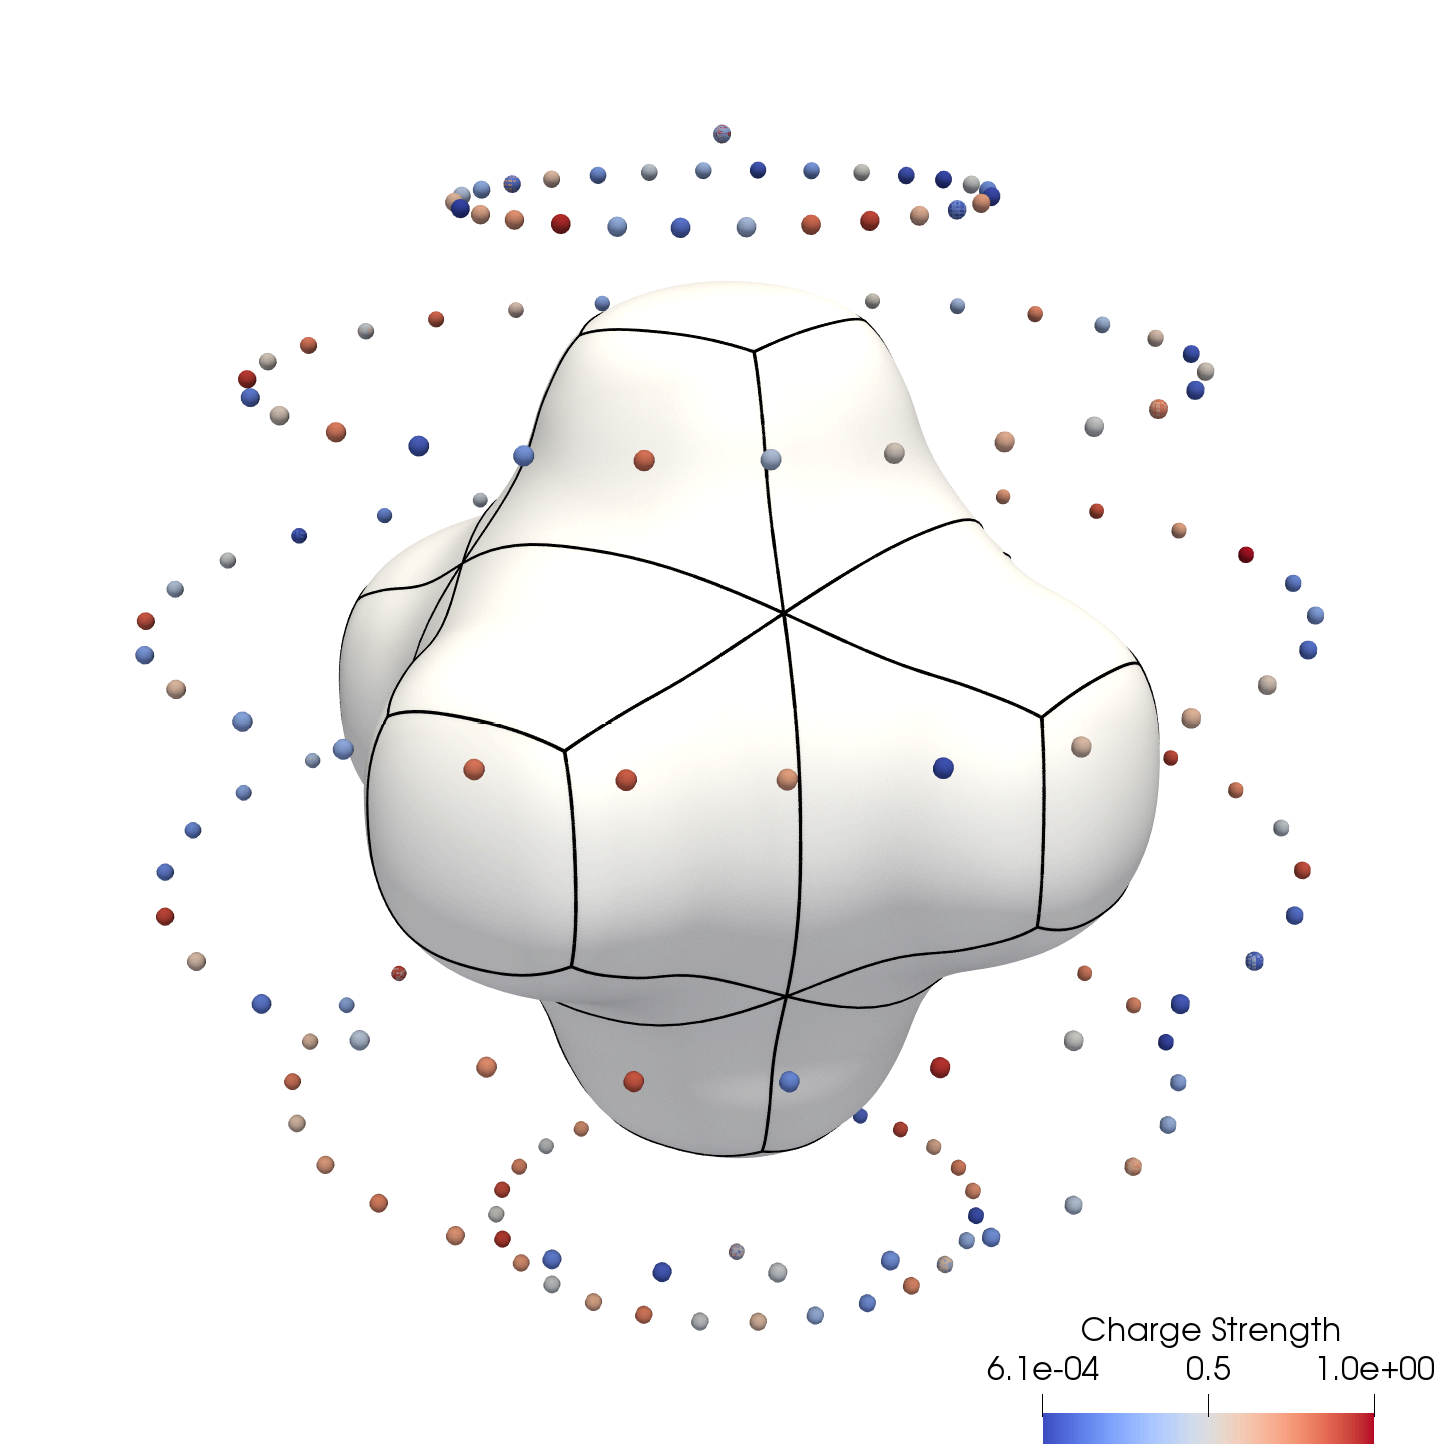
\includegraphics[width=.75\linewidth]{figs/pipe_convergence_setup}
  \end{minipage}\hfill
  \begin{minipage}{.5\textwidth}
      \centering
    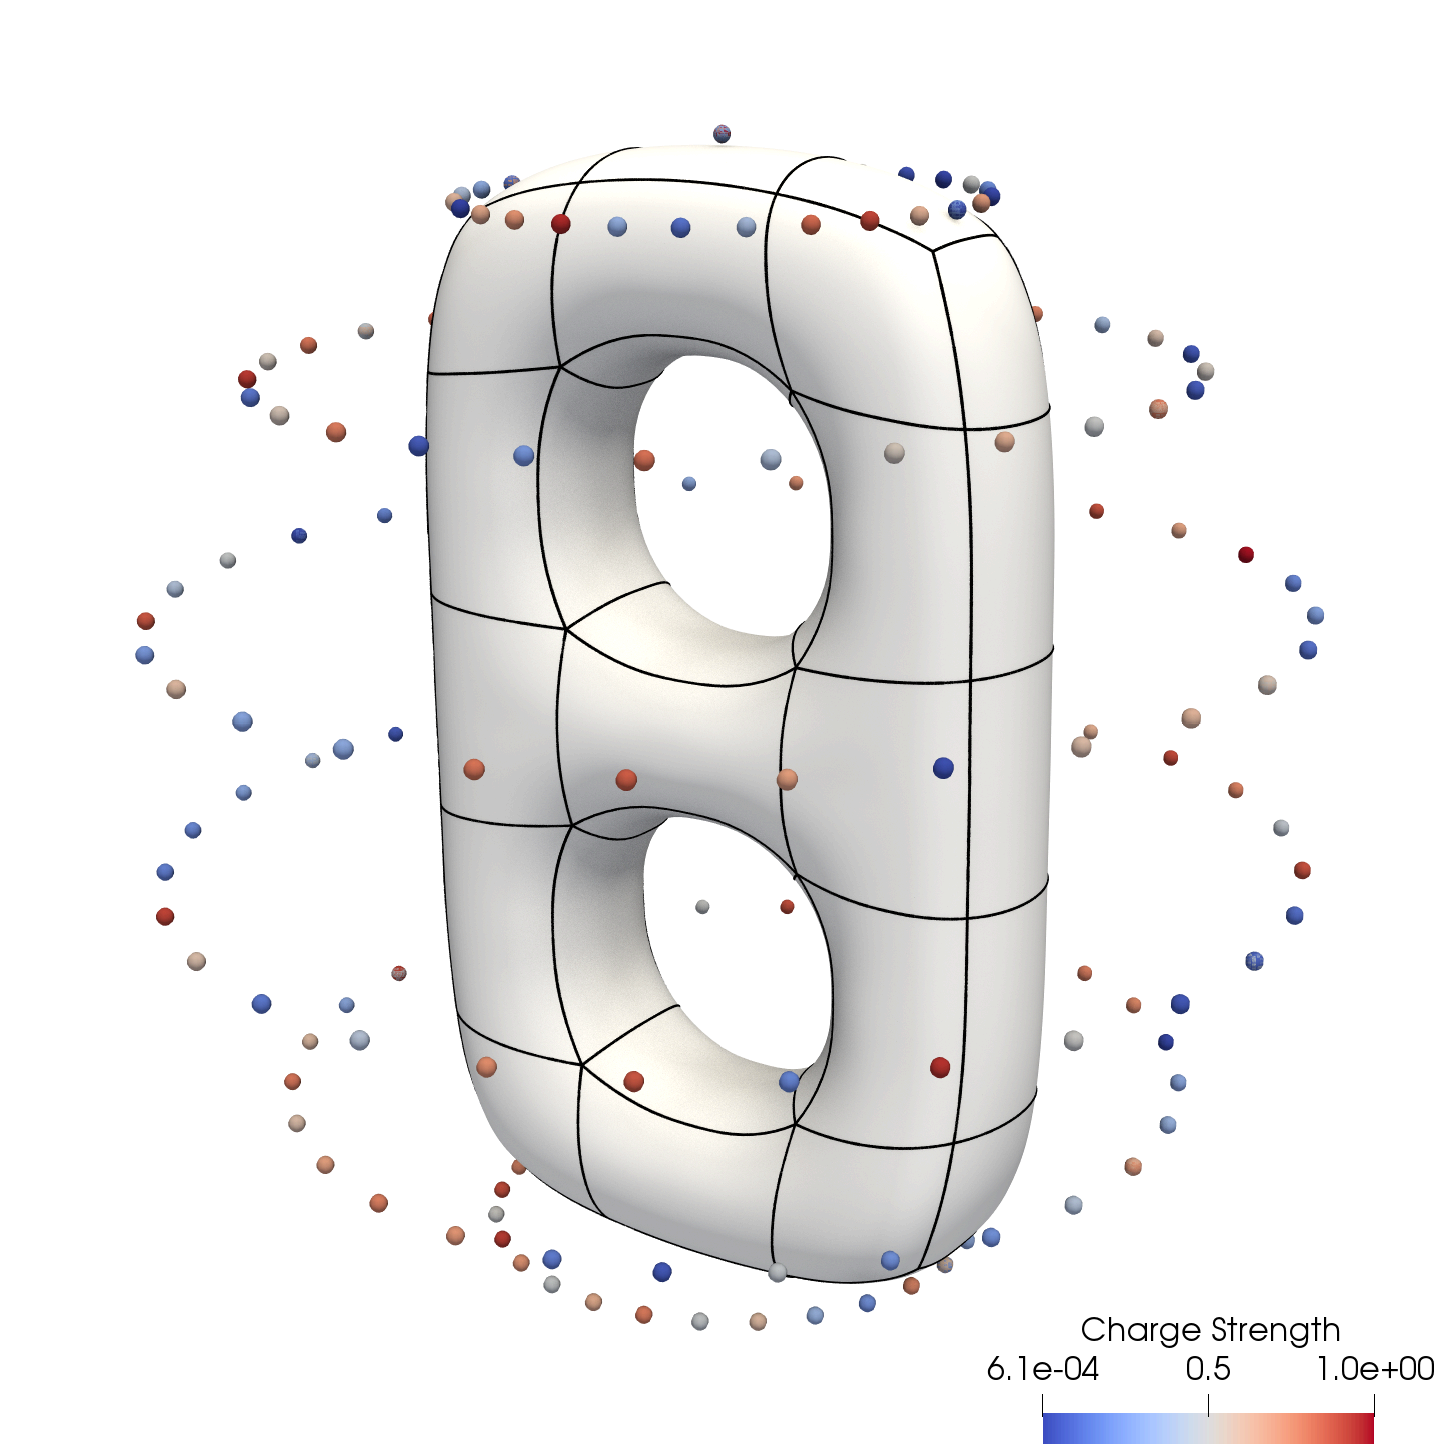
\includegraphics[width=.75\linewidth]{figs/ttorus2_convergence_setup}
  \end{minipage}\hfill
  \mcaption{fig:solver-conv-test-cases}{}{Geometry and singularities used for solver convergence tests. Figures are similar to \cref{fig:greens-id-test-cases}, but displaying geometries for testing the convergence of \qbkix within a \gmres solver.
  We use 30 16th-order polynomial patches for the pipe (left) and 50 20th-order patches for the genus two surface (right). 
  Note the proximity of the singularities to the domain of the genus two surface; the nearest singularity is less than $.05L$ from $\Gammah$.
}
\end{figure}

\begin{table}
\centering
\small
\setlength\tabcolsep{4pt}
\begin{tabular}{lllllll}
\toprule
{}Geometry & \pde &\multicolumn{4}{c}{Relative $\ell^\infty$ error (Number of patches)} & EOC\\
\midrule
Spheroid (\cref{fig:greens-id-test-cases}-left) & Laplace   &  $2.70\times 10^{-6 }$ (96) &  $1.92\times 10^{-7 }$ (384) &  $4.47\times 10^{-9 }$ (1536) &  $5.13\times 10^{-11 }$ (6144) & 5.35 \\
   \midrule
Pipe                                       & Laplace       &  $5.99\times 10^{-4 }$ (30) &  $3.03\times 10^{-5 }$ (120) &   $6.68\times 10^{-7 }$ (480) &  $2.27\times 10^{-8 }$ (1920) & 5.92\\
(\cref{fig:solver-conv-test-cases}-left)   & Elasticity    &  $7.17\times 10^{-2 }$ (30) &  $3.57\times 10^{-3 }$ (120) &   $8.90\times 10^{-5 }$ (480) &  $4.14\times 10^{-6 }$ (1920) & 5.45\\
                                           & Stokes        &  $8.53\times 10^{-2 }$ (30) &  $4.12\times 10^{-3 }$ (120) &   $1.03\times 10^{-4 }$ (480) &  $4.73\times 10^{-6 }$ (1920) & 5.43\\
   \midrule
Genus 2                                     & Laplace     &  $4.00\times 10^{-2 }$ (50) &  $1.25\times 10^{-4 }$ (200) &   $1.54\times 10^{-6 }$ (800) &  $5.73\times 10^{-10 }$ (3200) & 8.76 \\
(\cref{fig:solver-conv-test-cases}-right)   & Elasticity  &  $9.20\times 10^{-2 }$ (50) &  $1.05\times 10^{-3 }$ (200) &   $1.00\times 10^{-5 }$ (800) &  $9.44\times 10^{-8 }$ (3200) & 6.89\\
                                            & Stokes      &  $1.03\times 10^{-1 }$ (50) &  $1.18\times 10^{-3 }$ (200) &   $1.15\times 10^{-5 }$ (800) &  $1.03\times 10^{-7}$ (3200)& 6.88\\
\bottomrule
\end{tabular}
\mcaption{table:solver-data}{$\ell^\infty$ Relative error in \gmres solve and solution evaluation versus number of patches}{
  We solve \cref{eq:pde} by discretizing and evaluating the layer potential in the integral equation in \cref{eq:int-eq} as described in \cref{sec:singular-eval}.
  We use two-sided \qbkix inside of \gmres to solve for $\phi$, then evaluate \cref{eq:double_layer_disc} with one-sided \qbkix at a new set of points on $\Gammah$.
  Each column is the result of an additional level of uniform quadrisection of the patches in $\Pcoarse$. 
  The final column (EOC) is the estimated convergence order, computed via least-squares log-log fit of the error as a function of max patch size.
}
\end{table}

\begin{table}[!htb]
\centering
\small
\setlength\tabcolsep{8pt}
\begin{tabular}{llllll}
\toprule
{}Geometry & \pde &\multicolumn{4}{c}{Target points/second/core}\\
\midrule
%Cube                                    & Laplace         &  $2905$ &  $4124$ &  $4059$ &  $3979$ \\
Spheroid                                    & Laplace         &  $2737$ &  $3149$ &  $2846$ &  $2950$ \\
\midrule
%Pipe                                    & Laplace         &  $1894$ &  $3771$ &  $3757$ &  $4186$ \\
%(\cref{fig:greens-id-test-cases}-left)  & Elasticity      &  $361$  &  $451$ &   $459$  &  $480$  \\
%                                        & Stokes          &  $379$  &  $506$ &   $513$  &  $526$  \\
Pipe                                    & Laplace         &  $3046$ &  $2178$ &   $2832$  &  $2982$ \\
(\cref{fig:greens-id-test-cases}-left)  & Elasticity      &  $991$  &  $993$  &   $1189$  &  $1261$  \\
                                        & Stokes          &  $1048$ &  $1140$ &   $1335$  &  $1422$  \\
 \midrule
%Genus 2                                       & Laplace         &  $2542$  &  $3747$ &   $3895$  &  $4227$ \\
% (\cref{fig:greens-id-test-cases}-right)      & Elasticity      &  $350$  &  $531$ &   $553$  &  $564$ \\
%                                              & Stokes          &  $398$  & $587$ &   $638$  &  $X$ \\
Genus 2                                       & Laplace         &  $1862$ &  $2886$ &  $3122$  &  $2879$ \\
 (\cref{fig:greens-id-test-cases}-right)      & Elasticity      &  $729$  &  $1125$ &  $1255$  &  $1295$ \\
                                              & Stokes          &  $929$  &  $1304$ &  $1450$  &  $1504$ \\
\bottomrule
\end{tabular}
\mcaption{table:solver-perf-data}{Performance of singular evaluation in \gmres matrix-vector multiply}{
    For each test in \cref{table:solver-data}, we report the number of target points per second per core evaluated with two-sided \qbkix in a single \gmres matrix-vector multiplication.
}
\end{table}
We report the accuracy of the \qbkix scheme when used to solve \cref{eq:pde} via the integral equation in \cref{eq:int-eq}.
Two-sided \qbkix is used in the matrix-vector multiply inside \gmres to solve \cref{eq:int-eq} for the values of the density $\phi$ at the discretization points.
Then one-sided \qbkix is used to evaluate \cref{eq:double_layer_disc} at a slightly coarser discretization. 
Since \gmres minimizes the residual at the original discretization of \cref{eq:int-eq}, this final step prevents an artificially accurate solution by changing discretizations.
\cref{table:solver-data} lists the $\ell^\infty$ relative error values for the total solve and evaluation steps using \cref{sec:singular-eval} as we refine $\Pcoarse$ by subdivision as in the previous section.
In these tests, we choose $p=6$, $r= .005\sqrt{L}$ ($a = .005/\sqrt{L}$), and  $R= .03\sqrt{L}$ ($b = .03/\sqrt{L}$).
As for previous examples, we observe at least $5$th order convergence on all tested geometries in \cref{fig:solver-conv-test-cases} and \cref{fig:greens-id-test-cases}-left and all \pde's.
We include the spheroid example as an additional demonstration of a high accuracy solution via \gmres with our approach.
We report the number of target points evaluated per second per core with two-sided \qbkix in \cref{table:solver-perf-data}.
The results are similar to \cref{table:greens-id-perf-data}; the slower performance is because evaluation via two-sided \qbkix is more expensive than one-sided \qbkix.
\subsection{Comparison with \cite{YBZ}\label{sec:results-compare}}
In this section,  we compare our method to \cite{YBZ}, a previously proposed high-order, kernel-independent singular quadrature method in \threed for complex geometries. These characteristics are similar to  \qbkix shares these characteristics. \cite[Section 4]{morse2020bsupplementary} presents additional comparisons.

%To understand the performance of these two methods and see the implications of this complexity difference in practice, we now compare the performance of \qbkix with that of \cite{YBZ} on several concrete numerical examples.

The metric we are interested is \textit{cost for a given relative error}.
Assuming the surface discretization is $O(N)$, we measure the cost of a method as its total wall time during execution $T$ divided by the total wall time of an \fmm evaluation on the same $O(N)$ discretization, $T_\lbl{FMM}$. 
By normalizing by the \fmm evaluation cost, we minimize the dependence of the cost on machine- and implementation-dependent machine-dependent parameters.
%, such as clock speed, cache size, performance optimizations, etc.

We run the tests in this section on the spheroid geometry shown in \cref{fig:greens-id-test-cases}-left.
We focus on the singular quadrature scheme of \cite{YBZ}. 
The near-singular quadrature of \cite{YBZ} is algorithmically similar to \qbkix, but since an expensive singular quadrature rule is used as a part of near-singular evaluation, it has a higher total cost.
As a result, the accuracy and cost of near-singular evaluation of \cite{YBZ} is bounded by the accuracy and cost of the singular integration scheme.

To compare the full \qbkix method with \cite{YBZ}, we fit polynomial patches to the $C^\infty$ surface of \cite{ying2004simple}, denoted $\Gamma_b$, to produce $\Gammah$ during the first step of \cref{sec:admissible_algo}.
We apply the remaining geometry preprocessing algorithms of \cref{sec:admissible_algo} to $\Gammah$ to produce $\Pcoarse$.
After producing $\Pfine$ with two levels of uniform upsampling, we solve \cref{eq:int-eq} with two-sided \qbkix on $\Gammah$ and evaluate the solution on the boundary with one-sided \qbkix.
We then solve for the solution to \cref{eq:int-eq} on $\Gamma_b$ using \cite{YBZ}. 

For each of the tests in this section, we choose some initial spacing parameter
$h_0$ to discretize the surface of \cite{ying2004simple}, as in \cite{YBZ}, and use the $16\times$ upsampled grid and floating partition of unity radius proportional to $O(\sqrt{h})$, as in the original work.
We apply \qbkix to $\Gammah$ and the scheme of \cite{YBZ} to $\Gamma_b$ with spacing $h_0/2^i$, for $i=1,\hdots 4$.

As in the previous section, we choose the parameters $r$ and $R$ of \qbkix to be $O(\sqrt{L})$. 
For both quadrature methods, we use a multipole order of $16$ for \pvfmm with at most 250 points in each leaf box.
\begin{figure}[!htb]
  \centering
    \makebox[\textwidth][c]{ 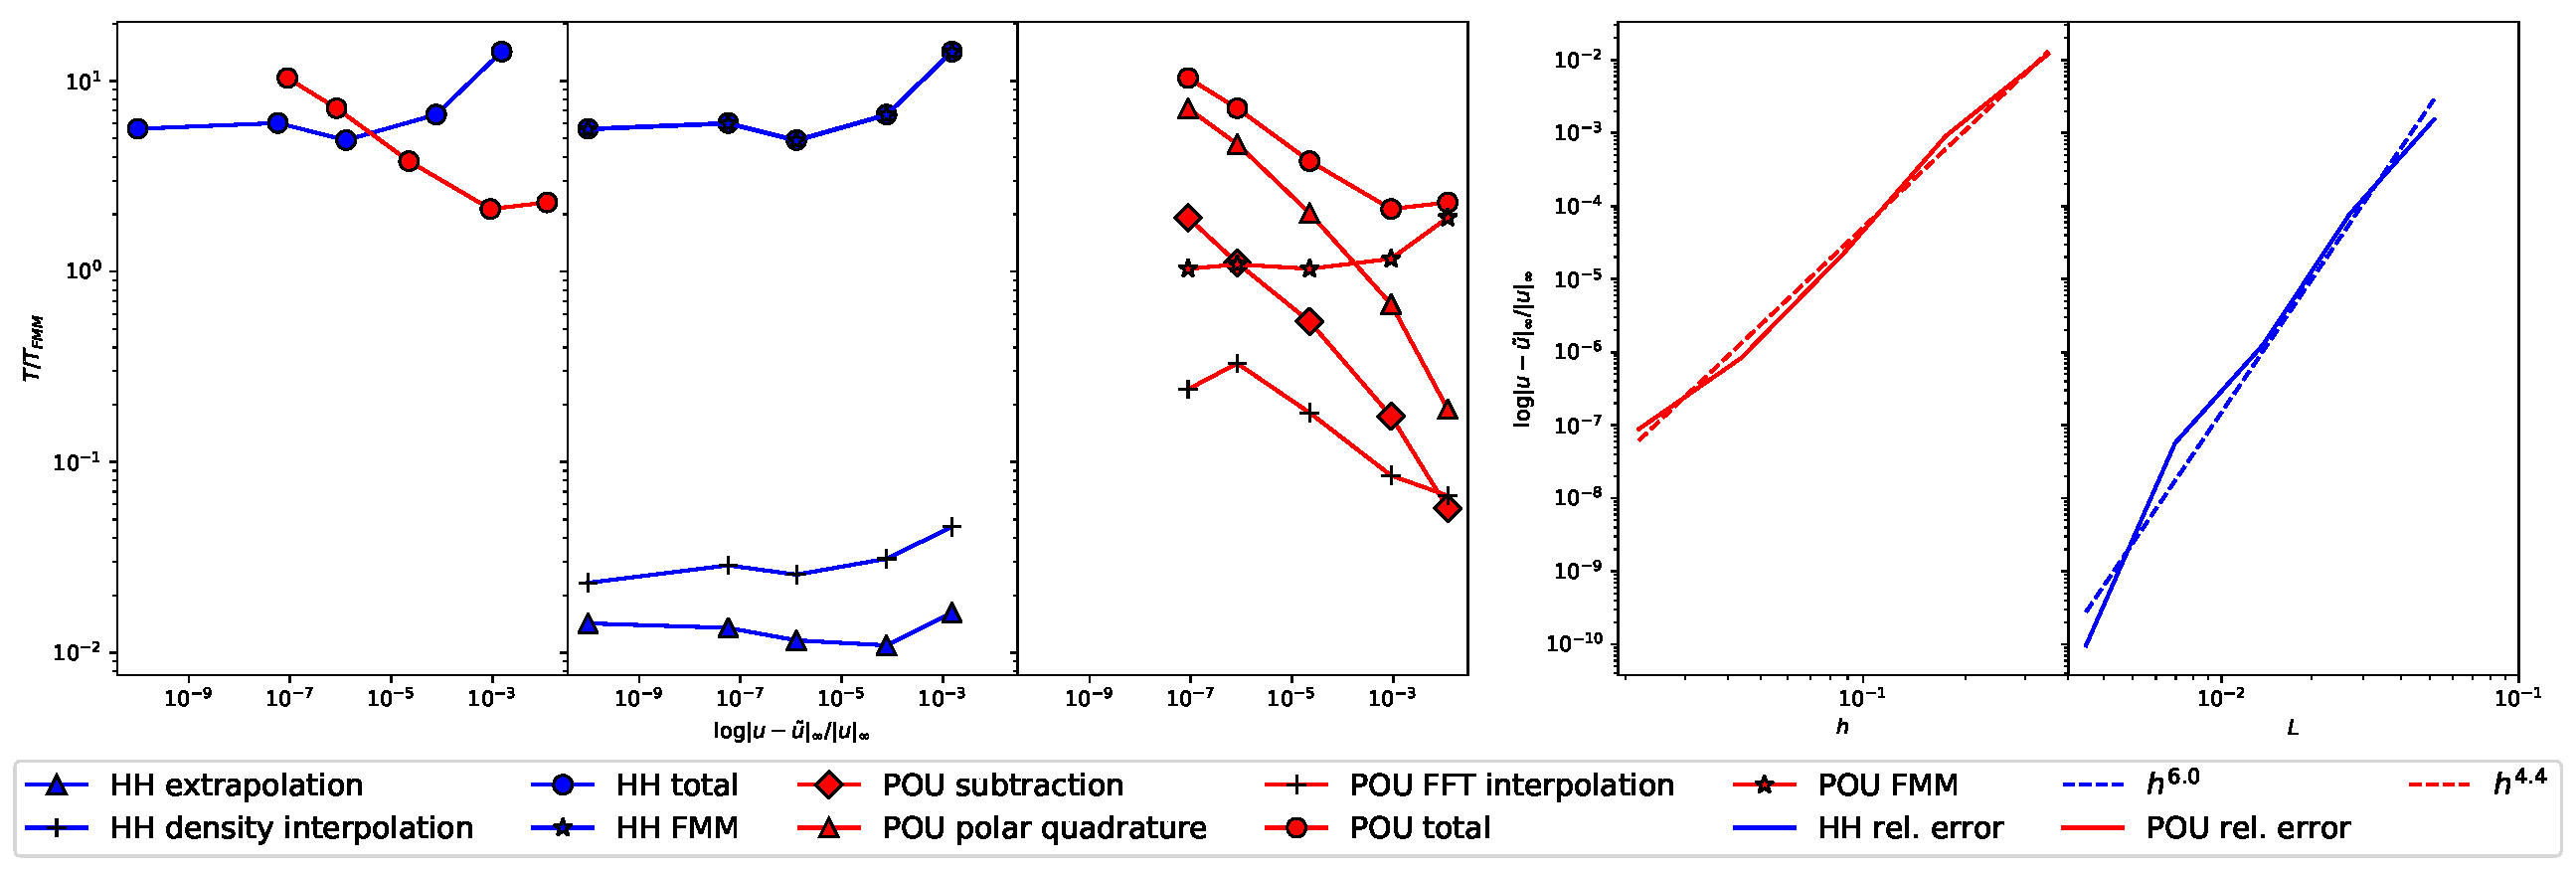
\includegraphics[width=1.1\textwidth]{figs/comparison_face_map_vs_blendsurf_cube_laplace_timing.pdf} }
    \makebox[\textwidth][c]{ 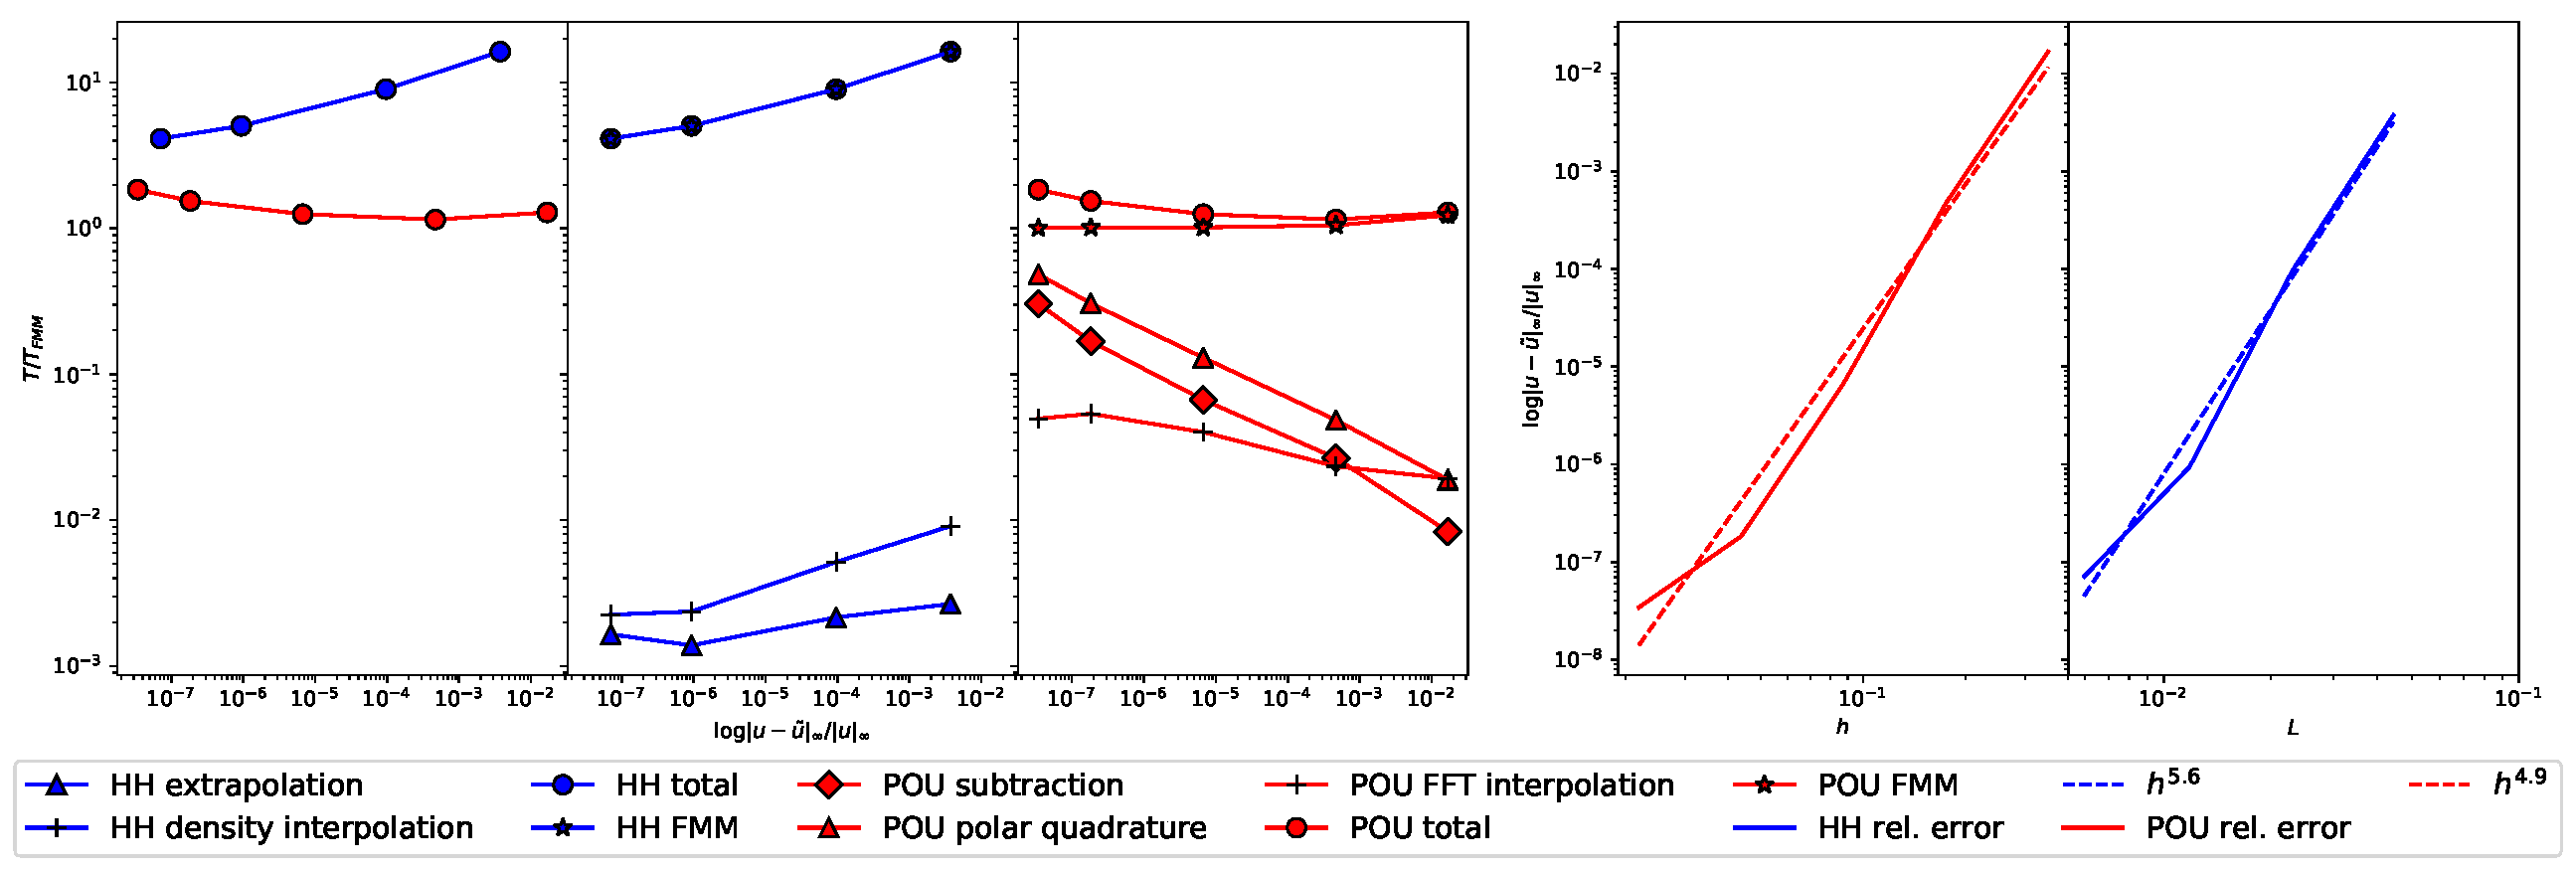
\includegraphics[width=1.1\textwidth]{figs/comparison_face_map_vs_blendsurf_cube_navier_timing.pdf} }
%  \hfill
%  \begin{minipage}{\textwidth}
%    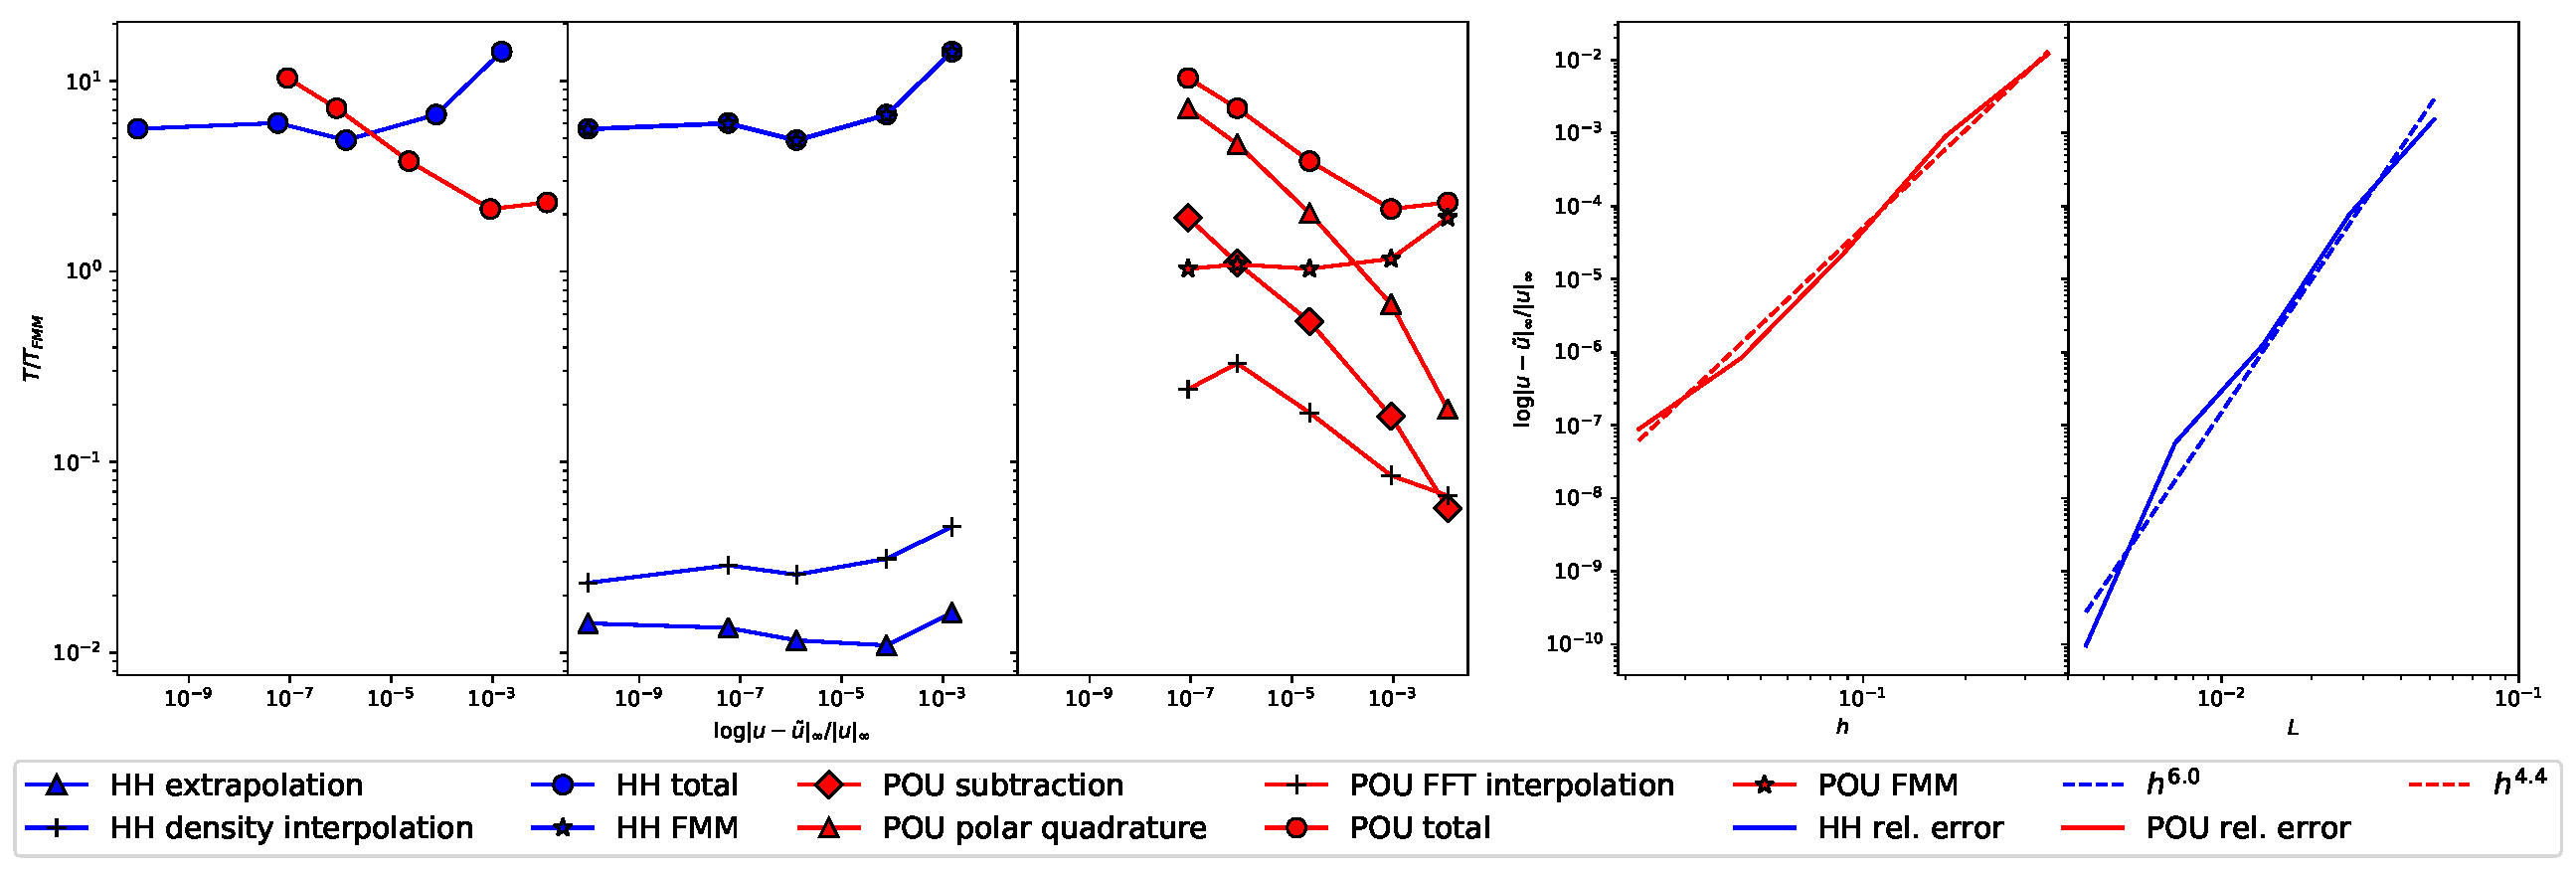
\includegraphics[width=\linewidth]{figs/comparison_face_map_vs_blendsurf_cube_laplace_timing.pdf}
%  \end{minipage}\hfill
%  \begin{minipage}{\textwidth}
%    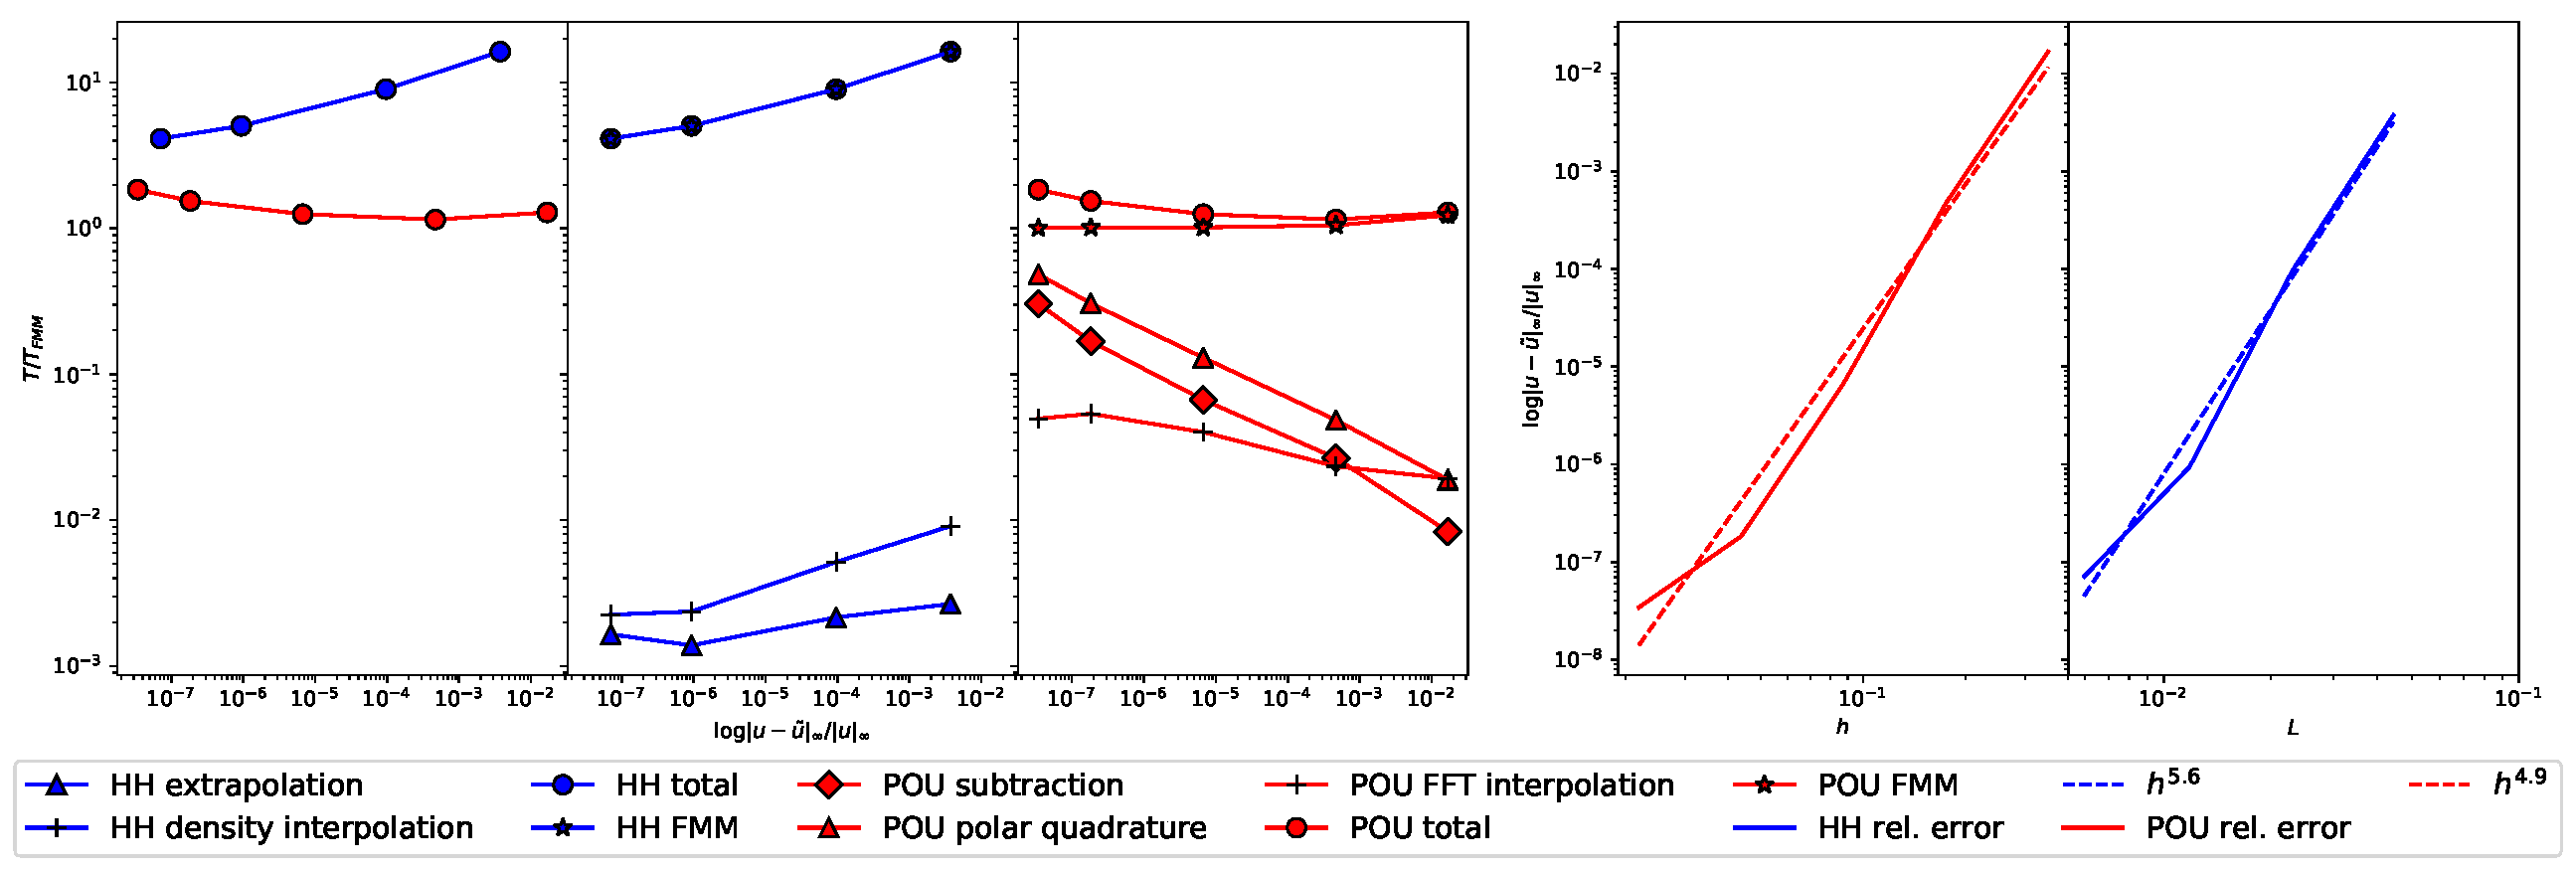
\includegraphics[width=\linewidth]{figs/comparison_face_map_vs_blendsurf_cube_navier_timing.pdf}
%  \end{minipage}\hfill
    \mcaption{fig:compare-solve-surface}{Comparison of \qbkix on polynomial patches (HH) versus \cite{YBZ} on the surface representation of \cite{ying2004simple} (POU) solving via \gmres for $u_c$}{
    Laplace (top) and elasticity (bottom) problems solved on the spheroid shown in \cref{fig:greens-id-test-cases}.
From left to right, we plot the total cost of each scheme, the cost of each subroutine for \qbkix (blue) and the singular quadrature scheme of \cite{YBZ} (red), and the relative error as a function of $h$.
    We plot error convergence of \cite{YBZ} as a function of $h$ and \qbkix as a function of $L$, due to the distinct discretizations.
    For \qbkix parameters, we choose $r=.013\sqrt{L}$, $R=.075\sqrt{L}$ for the Laplace problem; for the elasticity problem, we choose $r=.013\sqrt{L}$, $R=.08\sqrt{L}$. We choose $p=6$ and $q=15$ for both problems.
    For \cite{YBZ} the spacing is $h_0=.35$.
    Note that in the \qbkix timing breakdown, since the \fmm time is dominant, the \fmm cost lies directly on top of the total cost.
  }
\end{figure}
The results are shown in \cref{fig:compare-solve-surface}. 
From left to right, each plot details the total cost of each scheme, the cost of each subroutine for \qbkix (denoted \abbrev{HH}) and the singular quadrature scheme of \cite{YBZ} (denoted \abbrev{POU}), and the relative error as a function of $h$ and $L$, respectively, 
for all refinement levels. 
%Each data point in the plots, from right to left, is the result of $4\times $ finer sampling of the surfaces.
We plot the cost of both schemes the cost of each algorithmic step as a function of their computed relative error. 
In each figure, we present results for a Laplace problem (top) and an elasticity problem (bottom). % to highlight the difference in performance between scalar and vector kernels.

In \cref{fig:compare-solve-surface}, as expected, we observe a  higher  convergence rate for \qbkix compared to \cite{YBZ}. 
\cite{YBZ} outperforms \qbkix in terms of cost for all tested discretizations.  
%\DZ{For vector problems, the cost of additional \qbkix evaluations 
%for the problem size considered outweighs the savings from not using an asymptotically 
%more expensive singular quadrature.}
% This is due to the greater cost of a vector \fmm evaluation compared to a scalar one: the $m+p$  \fmm evaluation of \cite{YBZ} can be accelerated more efficiently with the method's small dense linear algebra computations.
 We observe that the \fmm evaluation in \cref{fig:compare-solve-surface} accounts for at least 95\% of the \qbkix cost.
This means that a local singular quadrature method (based on corrections to an \fmm evaluation, \cref{sec:related_work}) of \textit{worse} complexity can beat a global method, simply by virtue of reducing the \fmm size.
%Moreover, our implementation of \cite{YBZ} is not highly optimized, so we can expect a well-engineered \pou singular quadrature implementation such as \cite{malhotra2019taylor} to widen this gap.
By noting the large difference between the \qbkix \fmm cost and the \qbkix density interpolation, we can reasonably infer that a local \qbkix scheme should narrow this  performance gap and outperform \cite{YBZ} for larger problems, assuming that switching to a local scheme does not dramatically affect error convergence. 

%\qbkix is more efficient in the high-accuracy regime for Laplace problems, but \cite{YBZ} is more efficient for low-accuracy Laplace and elasticity problems.
%However, main difference from the previous section is that the crossover point in performance appears to be larger; \qbkix becomes more efficient than \cite{YBZ} around $10^{-5}$ and the gap between \qbkix and \cite{YBZ} for elasticity is less dramatic at $10^{-8}$.
%We attribute this improvement to the more efficient Clenshaw-Curtis discretization of \qbkix compared to the overlapping trapezoidal discretization of \cite{YBZ}.
%This is further supporting evidence that a local \qbkix implementation should surpass \cite{YBZ}.

\subsection{Requested target precision vs. computed accuracy}
\begin{figure}[!htb]
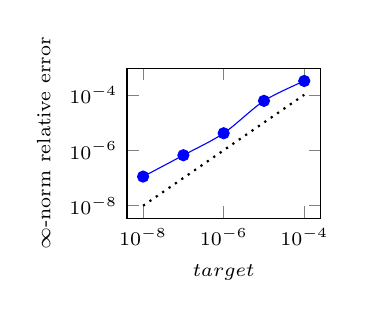
\begin{tikzpicture}
    \begin{loglogaxis}[
        xlabel=$\err{target}$,
        ylabel= $\infty$-norm relative error,
        ylabel near ticks,
        xlabel near ticks,
        label style={font=\scriptsize},
        tick label style={font=\scriptsize},
        width=.333\linewidth%7cm,height=3cm
    ]
    \addplot[smooth,mark=*,blue] plot coordinates {
        (1e-4,0.0003143683435301948)
        (1e-5,6.031924968205908e-05)
        (1e-6,4.103514547039301e-06)
        (1e-7,6.614064613404895e-07)
        (1e-8,1.122384348756594e-07)
    };
        \addplot[domain=1e-8:1e-4,dotted,thick]{x};

    \end{loglogaxis}
    \end{tikzpicture}
    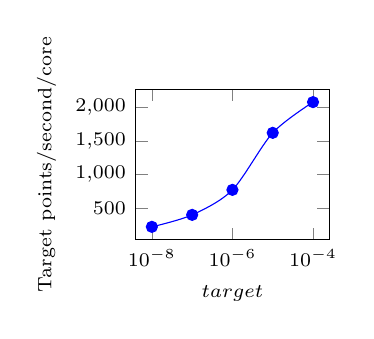
\begin{tikzpicture}
    \begin{semilogxaxis}[
        xlabel=$\err{target}$,
        ylabel= Target points/second/core,
        ylabel near ticks,
        xlabel near ticks,
        label style={font=\scriptsize},
        tick label style={font=\scriptsize},
        width=.333\linewidth%7cm,height=3cm
    ]
    \addplot[smooth,mark=*,blue] plot coordinates {
        (1e-4,2077)
        (1e-5,1620)
        (1e-6,772)
        (1e-7,400)
        (1e-8,222)
    };
    \end{semilogxaxis}
    \end{tikzpicture}
    \begin{tikzpicture}
    \begin{loglogaxis}[
        xlabel=$\err{target}$,
        ylabel= Number of patches,
        ylabel near ticks,
        xlabel near ticks,
        label style={font=\scriptsize},
        tick label style={font=\scriptsize},
        legend style={font=\tiny},
         legend image post style={scale=0.5},
        width=.333\linewidth%7cm,height=3cm
    ]
    \addplot[smooth,mark=*,blue] plot coordinates {
        (1e-4,128)
        (1e-5,128)
        (1e-6,128)
        (1e-7,128)
        (1e-8,128)
    };
    \addlegendentry{$|\Pcoarse|$}
    \addplot[smooth,mark=*,red] plot coordinates {
        (1e-4,5408)
        (1e-5,8288)
        (1e-6,28256)
        (1e-7,60032)
        (1e-8,113936)
    };
    \addlegendentry{$|\Pfine|$}
    \end{loglogaxis}
    \end{tikzpicture}
        \mcaption{fig:full-algo-perf}{Performance of full algorithm}{
            Left: $\infty$-norm relative error in singular integral vs requested target accuracy (blue). 
        The dotted line is the ideal behavior $y=x$.
        Middle: Performance in terms of target points evaluated per second per core with \qbkix.
        Right: Number of patches in $\Pcoarse$ and $\Pfine$ computed by the preprocessing algorithms.}
\end{figure}

In this section, we study the performance of the full algorithm outlined in \cref{sec:algo}.
We test \qbkix on the torus domain shown in \cref{fig:greens-id-test-cases}-right.
We choose a reference solution of the form of \cref{eq:point-charge-solution} with a single point charge located at the origin, in the middle of the hole of the torus.
We solve the integral equation with two-sided \qbkix and evaluate the singular integral on a distinct discretization with one-sided \qbkix.
We choose $q=20$, $p=6$ and $a=b/6$.
We select various values for $\err{target}$ using the plot in \cref{fig:extrap-err-p6} to choose $b$ to ensure sufficiently accurate extrapolation. 
We plot the results of our tests in \cref{fig:full-algo-perf}.

We see in \cref{fig:full-algo-perf}-left that we are consistently close to the requested target precision. 
We see a decline in target points per second per core as accuracy increases in \cref{fig:full-algo-perf}-middle.
This is explained by \cref{fig:full-algo-perf}-right, which shows an increase in the size $\Pfine$ as $\Pcoarse$ remains a fixed size.
The initial 128 patches in $\Pcoarse$ are enough to resolve the boundary condition and $\Gamma$, but we need greater quadrature accuracy for lower values of $\err{target}$ .
Decreasing the number of points in passed to the \fmm, i.e., decreasing the size of $\Pfine$, is the main way to improve performance of our method.
This is further indication that a local version of \qbkix will outperform a global approach.

\subsection{Full algorithm on interlocking torii\label{sec:results-torii}}
We now demonstrate the full algorithm pipeline on an exterior Laplace problem, whose boundary is defined by four interlocking torii shown in \cref{fig:torii}.
The domain boundary is contained in the box $[-3.8, 2.4] \times [-1.1, 1.1] \times [-1,1]$.
The shortest distance between two adjacent torii is less than 10\% of a polynomial patch length defining the boundary.
We again use a boundary condition of the form \cref{eq:point-charge-solution} with a single point charge located at $(0,.03,.875)$, inside the upper half of the second torus from the right in \cref{fig:torii}.
This problem is challenging due to the nearly touching geometry of the torii, along with the singularity placed close to the boundary.
We run the admissibility and adaptive upsampling algorithms outlined in \cref{sec:algo}, solve \cref{eq:int-eq} using two-sided \qbkix, and evaluate the solution on the boundary using one-sided \qbkix.
The absolute error in the $\infty$-norm of the singular evaluation is plotted on the boundary surface.

\begin{figure}[!htb]
  \centering
  \hfill
  \begin{minipage}{.65\textwidth}
    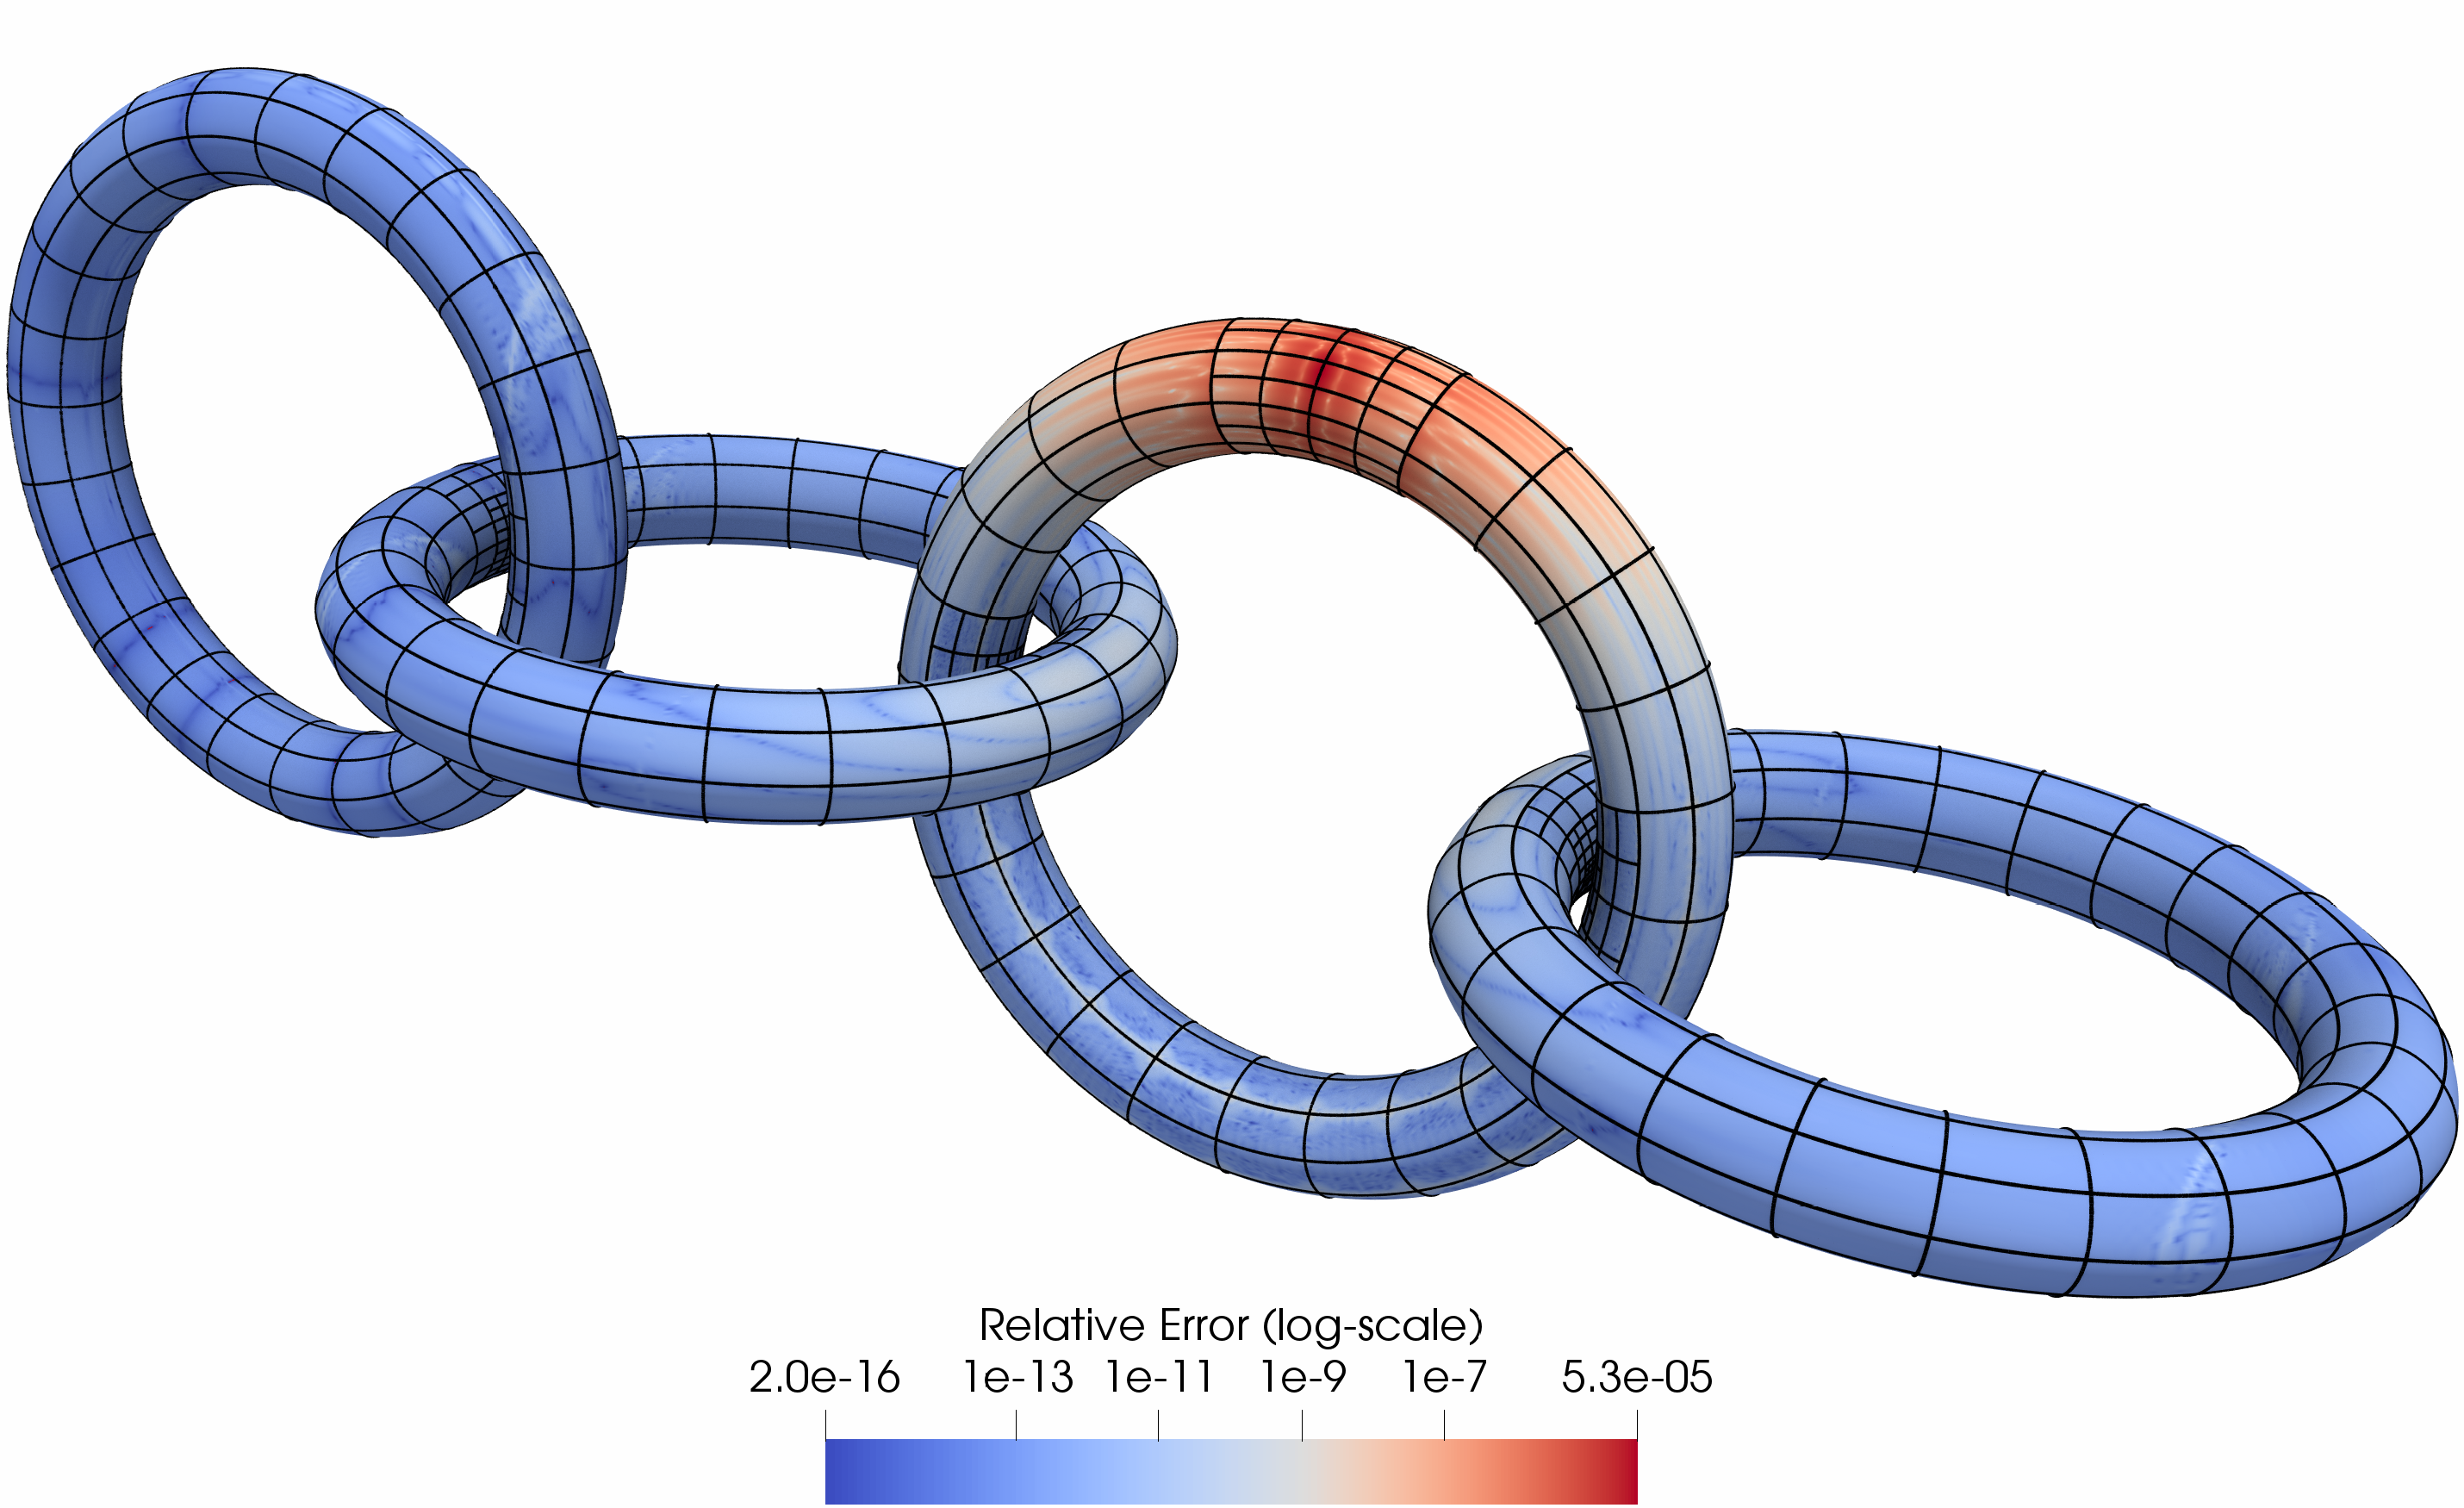
\includegraphics[width=\linewidth]{figs/interlocking_torus_error.png}
  \end{minipage}\hfill
  \begin{minipage}{.35\textwidth}
    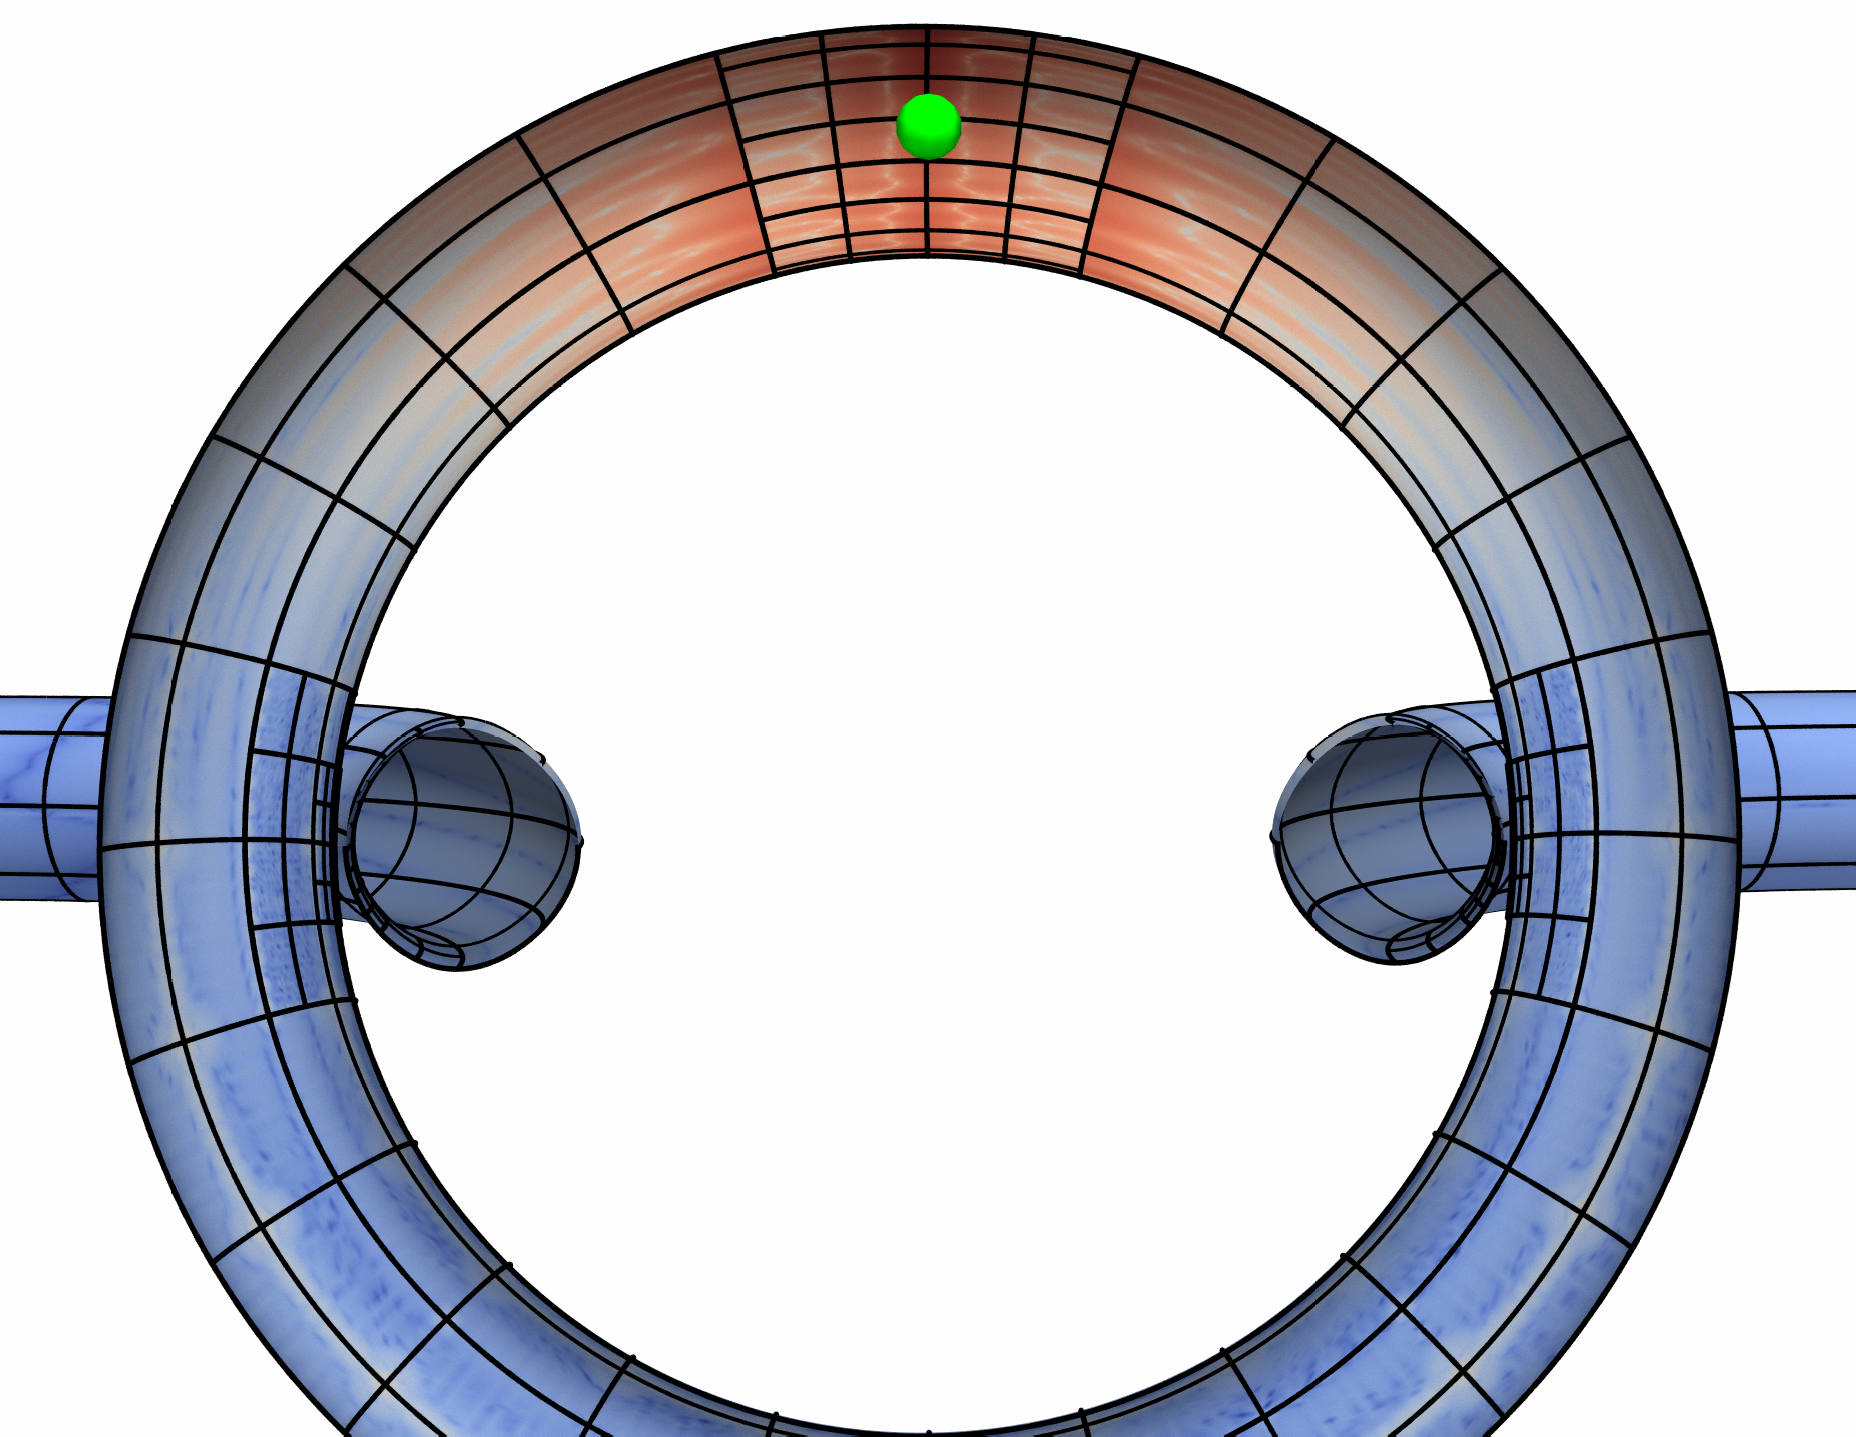
\includegraphics[width=\linewidth]{figs/interlocking_torus_error_cross_section.png}
  \end{minipage}\hfill
  \mcaption{fig:torii}{Absolute error of \gmres solve via \qbkix on interlocking torii}{Left: The admissible set of 1128 patches in $\Pcoarse$ used to solve \cref{eq:int-eq} is shown (black lines denote patch boundaries).
  The point charge generated the boundary condition is located within the second torus from the right. 
    Right: a cross-section of the torii geometry through the $xz$-plane, showing the second torus from the right and the location of the singularity (green point).
}
\end{figure}
Using $a=.1$, $b=.025$, $p=6$ and $q=20$, we achieve a maximum pointwise error of $1.29\times 10^{-5}$. 
\gmres was able to reduce the residual by a factor of $10^{-13}$ over 109 iterations.
There are 288768 quadrature points in the coarse discretization, 18235392 quadrature points in the fine discretization, and 3465216 check points used in the two-sided \qbkix evaluation inside \gmres.
We evaluate the solved density at 451200 points on the boundary with one-sided \qbkix to produce the render in \cref{fig:torii}.
On a machine with two Intel Xeon E-2690v2 3.0GHz \abbrev{CPU}'s, each with 10 cores, and 100 \abbrev{GB} of \abbrev{RAM},
the \gmres solve and interior evaluation required 5.7 hours and can evaluate the singular integral at a rate of 1709 target points per second per core.


\subsection{Solution on complex geometry\label{sec:results-blood-vessel}}

\begin{figure}[!htb]
  \centering
  \hfill
  \begin{minipage}{.7\textwidth}
    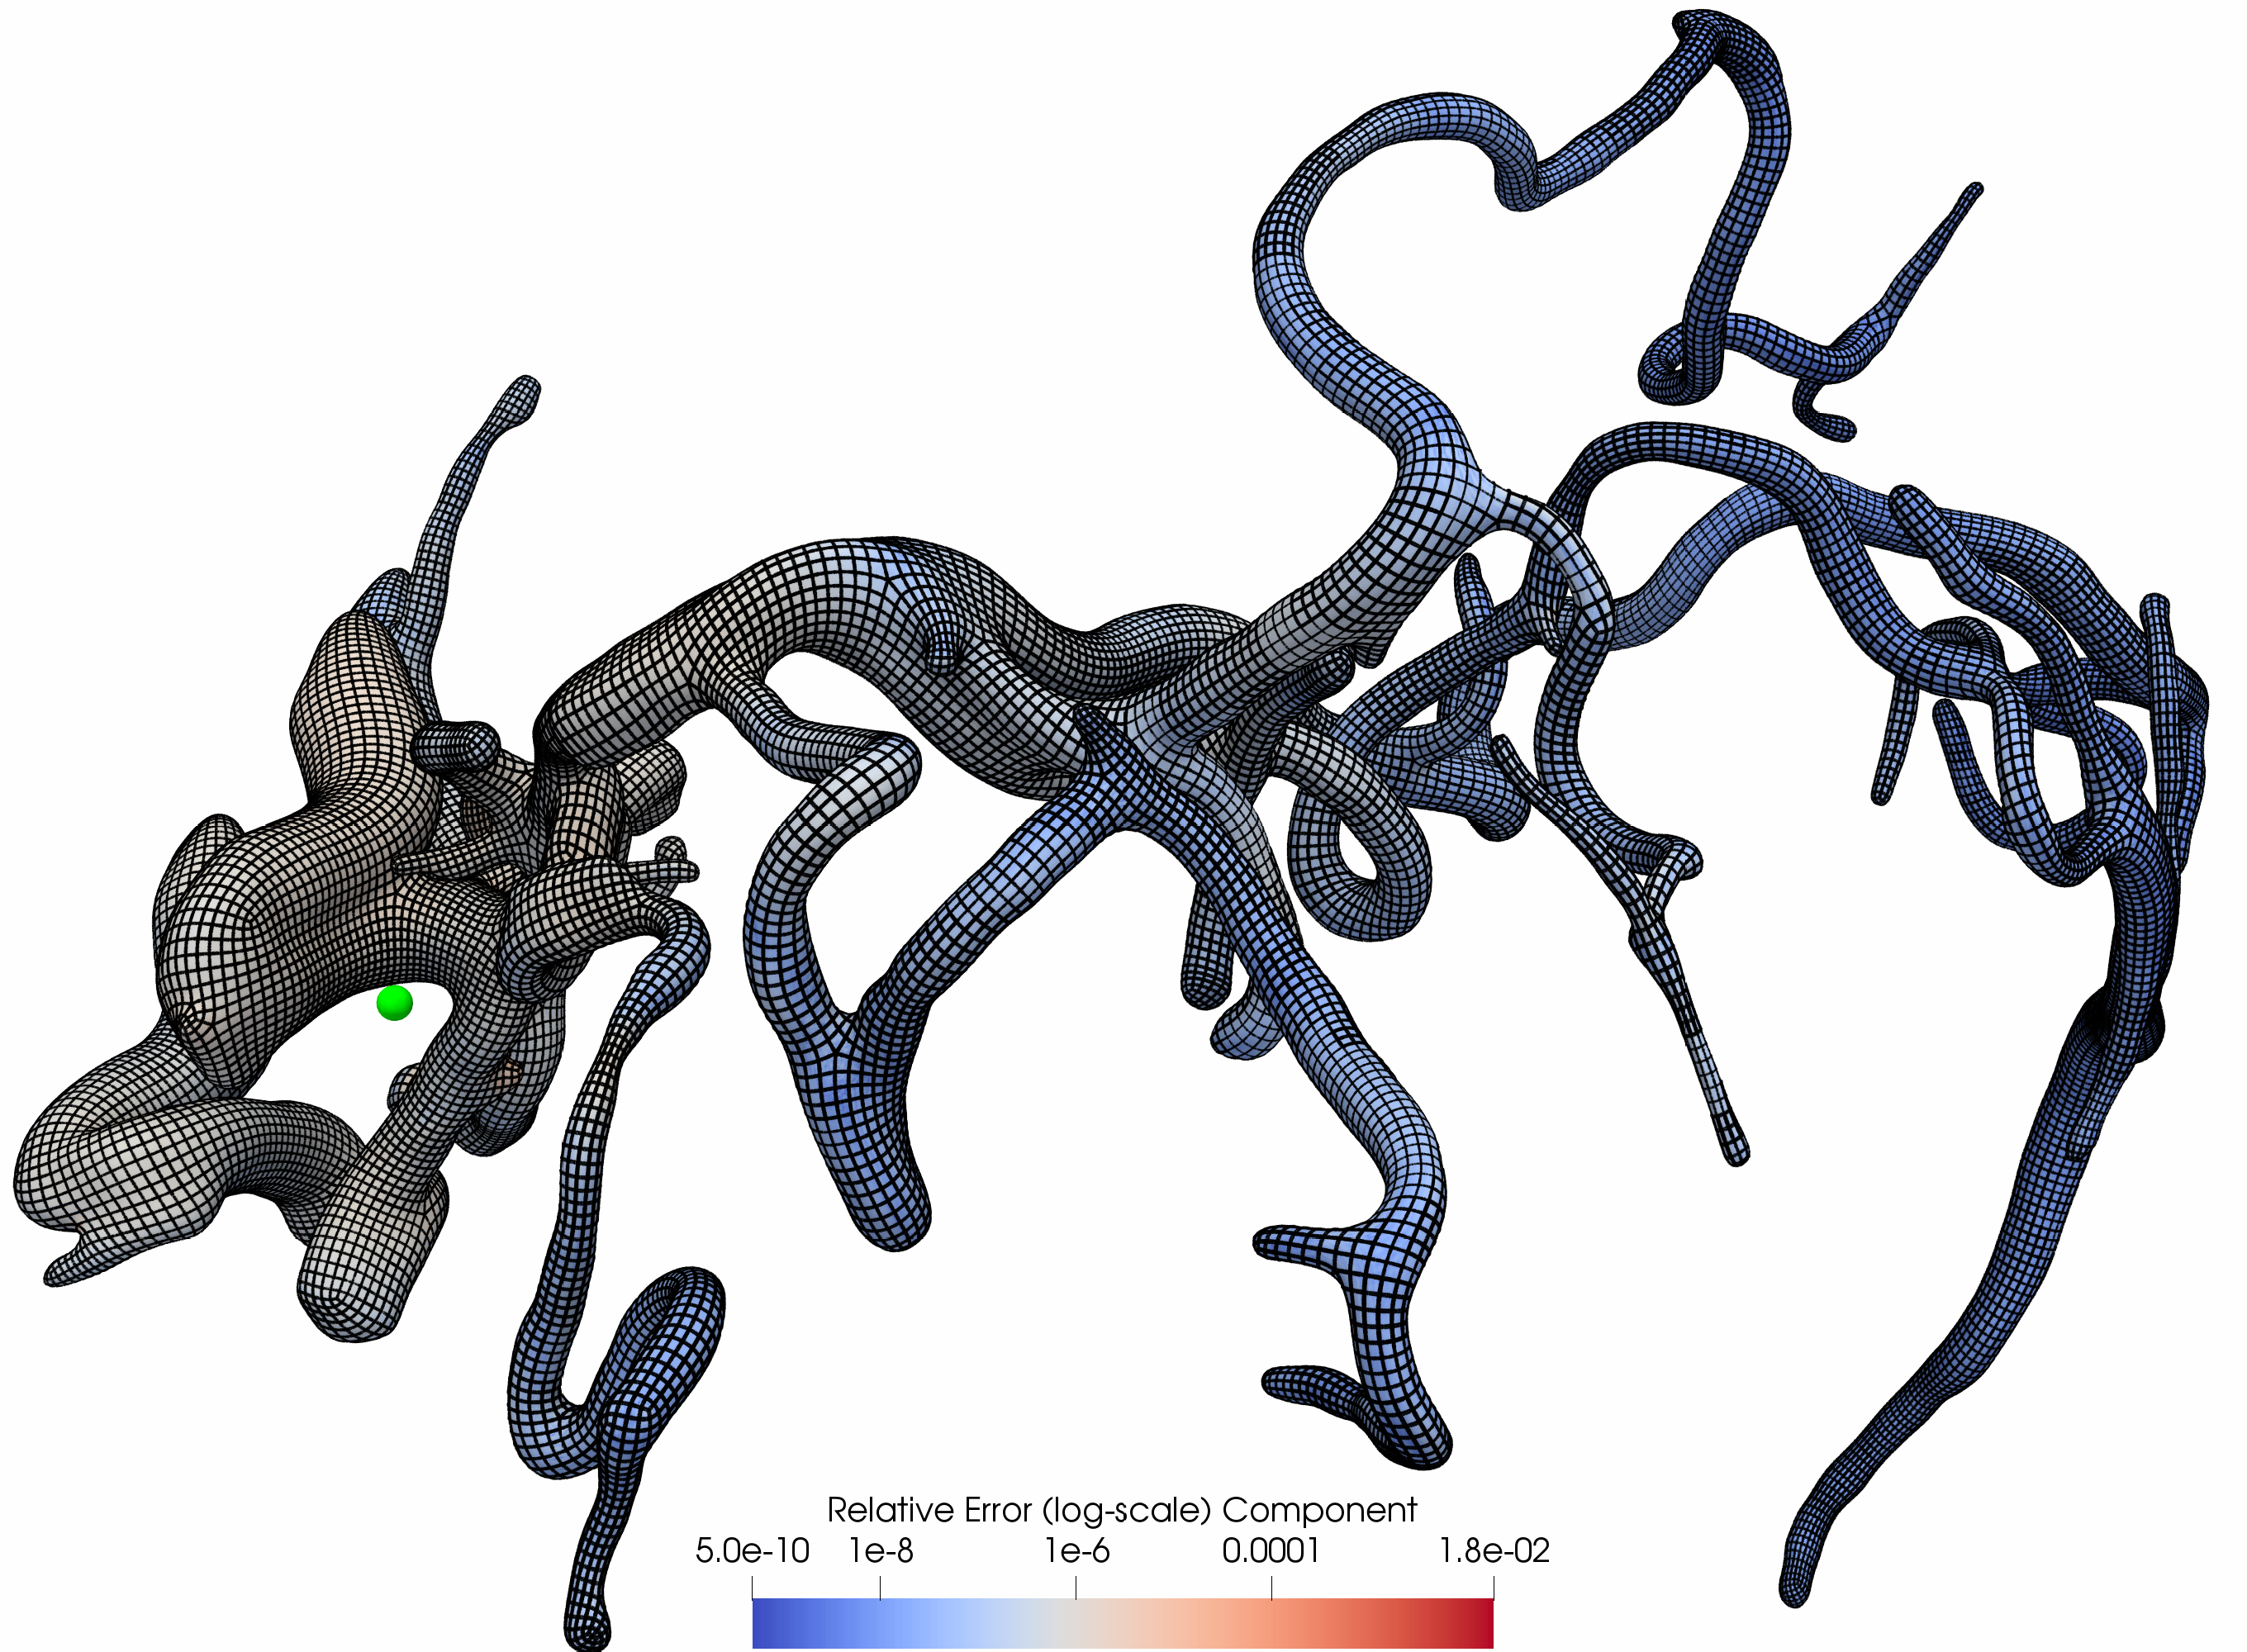
\includegraphics[width=\linewidth]{figs/largest_vessel_section.png}
  \end{minipage}\hfill
  \mcaption{fig:vessel}{Absolute error of \gmres solve via \qbkix on complex blood vessel geometry used in \cite{lu2019scalable}}{The blood vessel uses 40,960 8th order polynomial patches (black edges denote patch boundaries). The geometry is admissible by construction. 
    The point charge is located on left side of the figure (green)}
\end{figure}

We have demonstrated in \cite{lu2019scalable} a parallel implementation of \cref{sec:singular-eval}, applied to simulating red blood cell flows.
The surface geometry of the blood vessel shown in \cref{fig:vessel} is complex, with rapidly varying curvatures and geometric distortions due to singular vertices in the surface mesh.
Since the surface is admissible, we are able to apply parallel \qbkix directly without geometric preprocessing to solve an interior Dirichlet Stokes problem.
We use $a=.125$, $b=.125$, $p=6$ and $q=16$ as simulation parameters.

Using 32 machines each with twenty 2.6 Ghz cores with 100\abbrev{GB} of \abbrev{RAM}, we achieve a maximum pointwise error of $3\times 10^{-6}$ when solving a Stokes problem with constant density. 
We then place a random vector point charge two patch lengths away (relative to the patches in $\Pcoarse$) from the domain boundary (on the left side of \cref{fig:vessel}, solve \cref{eq:int-eq} using two-sided \qbkix, and evaluate the solution on the boundary using one-sided \qbkix.
The absolute error in the $\infty$-norm of the singular evaluation is plotted on the boundary surface.
There are 10,485,760 quadrature points in the coarse discretization, 167,772,160 quadrature points in the fine discretization, and 125,829,120 check points used in the two-sided \qbkix evaluation inside \gmres.
We evaluate the solved density at 209,715,200 points on the boundary with one-sided \qbkix to produce the render in \cref{fig:torii}.
We achieve a maximum pointwise error of $1.8\times 10^{-2}$ and can evaluate the singular integral at rate of 3529 target points per second per core. 
%The \gmres solve with two-sided \qbkix converged to \note[MJM]{X} in \note[MJM]{Y} iterations in \note[MJM]{Z} hours.

